%\documentclass[Serif, 10pt, brown, handout]{beamer} % Disable overlays for handout format
%\documentclass[Serif, 10pt, brown, handout, notes]{beamer} % Disable overlays for handout format and print notes
\documentclass[Serif, 10pt, brown]{beamer}
\usepackage{booktabs,xcolor}
%\usepackage[svgnames,table]{xcolor}
%\usepackage[tableposition=above]{caption}
\usepackage{pifont}
\newcommand*\CHECK{\ding{51}}
\usepackage{array}
\newcolumntype{P}[1]{>{\centering\arraybackslash}p{#1}}
\usepackage{tabto}
\usepackage{listings}
\usepackage{xmpmulti}
\usepackage{media9}
%
\usepackage{setspace,mathtools,amssymb,multirow,array,amsmath,tikz}
\usepackage[normalsize]{subfigure}
\usetikzlibrary{patterns}
\usetikzlibrary{automata,positioning,decorations.pathreplacing,decorations}

\usepackage{curves}
\usepackage{wasysym}
\usepackage{epsfig,epstopdf,graphicx}

\curvewarnfalse
%
\newtheorem{proposition}{Proposition}
\theoremstyle{example}
\newtheorem{theoremh}{Theorem}
\theoremstyle{plain}
\renewcommand{\textfraction}{0.01}
\renewcommand{\floatpagefraction}{0.99}
\newcommand{\ul}{\underline}
\newcounter{units}
%
\usepackage[round]{natbib}
 \bibpunct[, ]{(}{)}{,}{a}{}{,}%
 \def\bibfont{\small}%
 \def\bibsep{\smallskipamount}%
 \def\bibhang{24pt}%
 \def\newblock{\ }%
 \def\BIBand{and}%
%
\setbeamercovered{dynamic}
% Logo
\logo{
\includegraphics[width=0.625in,keepaspectratio]{unipv.jpeg}}
%
% Setup
\mode<presentation>
	{
\usetheme[right,currentsection, hideothersubsections]{UTD}
			\useoutertheme{sidebar} \useinnertheme[shadow]{rounded}
			\usecolortheme{whale} \usecolortheme{orchid}
			\usefonttheme[onlymath]{serif}
			\setbeamertemplate{footline}{\centerline{Slide \insertframenumber/\inserttotalframenumber}}
	}
%

% Title
\usebeamercolor[fg]{author in sidebar}
\subtitle{Problem Solving in Fisica}
\title[{Sistema Solare}]{\sc Simulazione Sistema Solare}
\author[\ul{Mauro Ghirardi}]{{\bf Mauro Ghirardi}}
\institute[UTD]{\sc\small Università degli Studi di Pavia}
\date[UCI]{Giugno 2025}
%%

%Presentation
\begin{document}
\frame{\titlepage}
%

%Slides

%TOC

% Introduction
\section[Intro]{Introduzione}
    \begin{frame}
        \frametitle{Contenuti}
        \transblindsvertical
        \tableofcontents[currentsection]
    \end{frame}

\setbeamercolor{background canvas}{use=structure,bg=white}
\setbeamercolor{background}{use=structure,bg=white}

    \begin{frame}{Il sistema solare}
        \begin{block}{Descrizione fisica}
            N corpi di massa $m_i$ che interagiscono secondo la legge di gravitazione universale $\Rightarrow$ N equazioni differenziali del secondo ordine accoppiate
            \\
            \begin{equation}
                \vec{a_i} = -\sum_{i\neq j}\frac{Gm_j}{r_{ij}^2}\frac{\vec r_{ij}}{r_{ij}}\,\,\,\,\,\,\,\,\forall i=1,\dots N
            \end{equation}
        \end{block}
    
        \begin{figure}
            \centering
            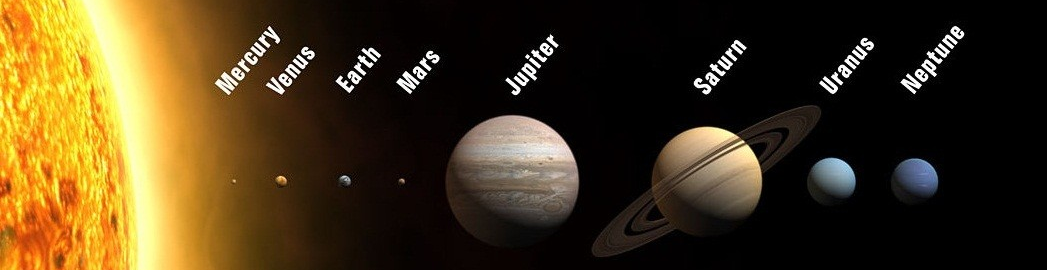
\includegraphics[width=\textwidth]{1_intro/siss.png}
            %\caption{Caption}
            %\label{fig:enter-label}
        \end{figure}       
    \end{frame}

    \begin{frame}{Il progetto}
        \begin{block}{Valutazione della coerenza della simulazione}
            \begin{enumerate}
                \item Studio delle quantità "conservate":
                \begin{itemize}
                    \item Energia totale
                    \item Momento angolare totale
                    \item eccentricità dell'orbita
                    \item distanza dal sole
                    \item inclinazione dell'orbita
                \end{itemize}
                \item Studio della dipendenza dai parametri:
                \begin{itemize}
                    \item Posizione e velocità dei corpi
                    \item Tempo di simulazione
                    \item Granularità
                    \item Metodo di approssimazione
                \end{itemize}              
            \end{enumerate}
        \end{block}

        \begin{block}{Efficienza}
            \begin{enumerate}
                \item Confronto tra C++ e Python
                \item Utilizzo dei due linguaggi per scopi differenti
            \end{enumerate}
        \end{block}
        
    \end{frame}


% code
\section[Code]{Codice}
    \begin{frame}
        \frametitle{Contenuti}
        \transblindsvertical
        \tableofcontents[currentsection]
    \end{frame}
    
    \begin{frame}{Architettura del codice}
        \begin{figure}
            \centering
            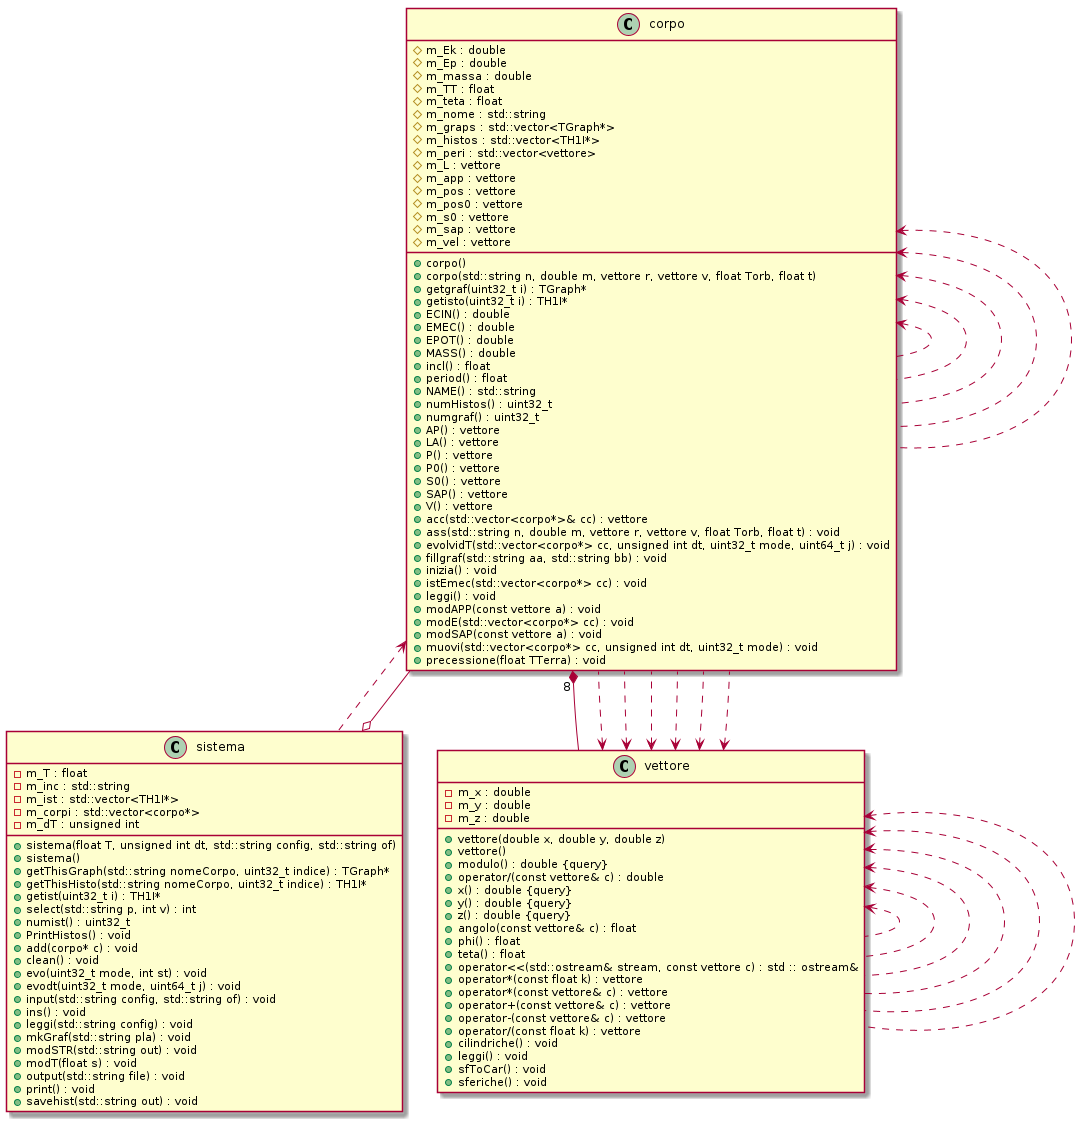
\includegraphics[width=\textwidth, height=6cm]{tutto.png}
            \label{fig:uml}
        \end{figure}
    \end{frame}
    
        \subsection[Approx]{Aprrossimazione}
        
        \begin{frame}{Gestione evoluzione}
            Funzione sistema::evo() - loop sul tempo
            \begin{itemize}
                \item[$\Rightarrow$] Funzione sistema::evodt() - loop sui corpi
                \begin{itemize}
                    \item[$\Rightarrow$] Funzione corpo::edolvidt() - aggiornamento posizione/velocità e raccolta dati per ogni corpo
                    \begin{itemize}
                        \item[$\Rightarrow$] Funzione corpo::muovi() - scelta metodo di approssimazione
                    \end{itemize}
                \end{itemize}
            \end{itemize}    

            \begin{exampleblock}{$N>2 \Rightarrow$ Soluzione approssimata tramite metodi iterativi discreti:}
                \begin{enumerate}
                    \item Metodo di Eulero - approssimazione lineare
                \end{enumerate}
                \begin{equation}
                \left\{ 
                \begin{array}{l}
                    \vec{a_i}(t)=f_{GravUniv}(\vec{x_i}(t)) \\
                    \vec{v_i}(t+\Delta t)=\vec{v_i}(t)+\vec{a_i}\Delta t \\
                    \vec{x_i}(t+\Delta t)=\vec{x_i}(t)+\vec{v_i}(t+\Delta t)\Delta t
                \end{array}
                \right.
                \end{equation}
            \end{exampleblock}
        \end{frame}

        \begin{frame}{Gestione evoluzione}
            Funzione sistema::evo() - loop sul tempo
            \begin{itemize}
                \item[$\Rightarrow$] Funzione sistema::evodt() - loop sui corpi
                \begin{itemize}
                    \item[$\Rightarrow$] Funzione corpo::edolvidt() - aggiornamento posizione/velocità e raccolta dati per ogni corpo
                    \begin{itemize}
                        \item[$\Rightarrow$] Funzione corpo::muovi() - scelta metodo di approssimazione
                    \end{itemize}
                \end{itemize}
            \end{itemize}    

            \begin{exampleblock}{$N>2 \Rightarrow$ Soluzione approssimata tramite metodi iterativi discreti:}
                \begin{enumerate}
                    \item Metodo di Eulero - approssimazione lineare
                    \item Runge-Kutta $2^{nd}$ order - Eulero modificato
                \end{enumerate}
                \begin{equation}
                \left\{ 
                \begin{array}{l}
                    \vec{a_i^1}(t)=f_{GravUniv}(\vec{x_i}(t)) \\
                    \vec{x'}(t+\Delta t)=\vec{x_i}(t)+\vec{v_i}(t)\Delta t \\
                    \vec{a_i^2}(t)=f_{GravUniv}(\vec{x'}(t)+\Delta t) \\
                    \vec{v_i}(t+\Delta t)=\vec{v_i}(t)+\frac{\vec{a_i^1}+\vec{a_i^2}(t)}{2}\Delta t \\
                    \vec{x_i}(t+\Delta t)=\vec{x_i}(t)+\frac{\vec{v_i}(t)+\vec{v_i}(t+\Delta t)}{2}\Delta t
                \end{array}
                \right.
                \end{equation}
            \end{exampleblock}
        \end{frame}

        \begin{frame}{deltaT=3600s}
            \begin{columns}
                \column{.4\textwidth}
                \centering
                %\caption{Momento angolare del sistema dopo 2 anni nei due metodi descritti}            
                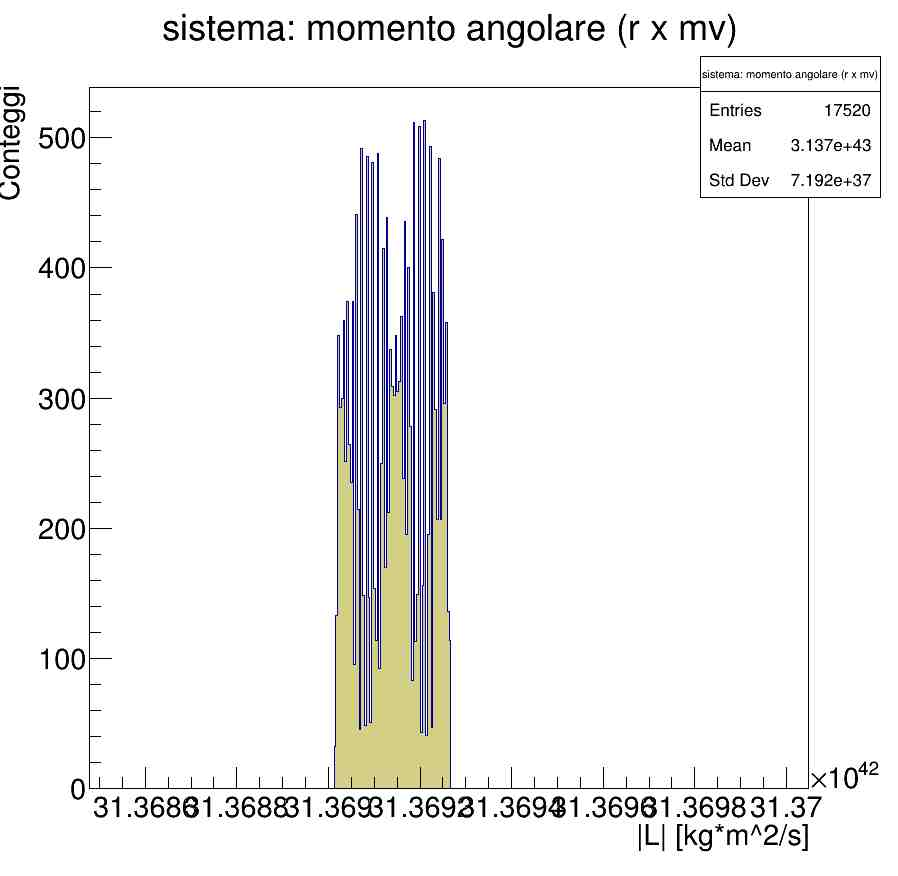
\includegraphics[width=4cm,height=4cm]{2_approx/L_2_0.jpg}\\
                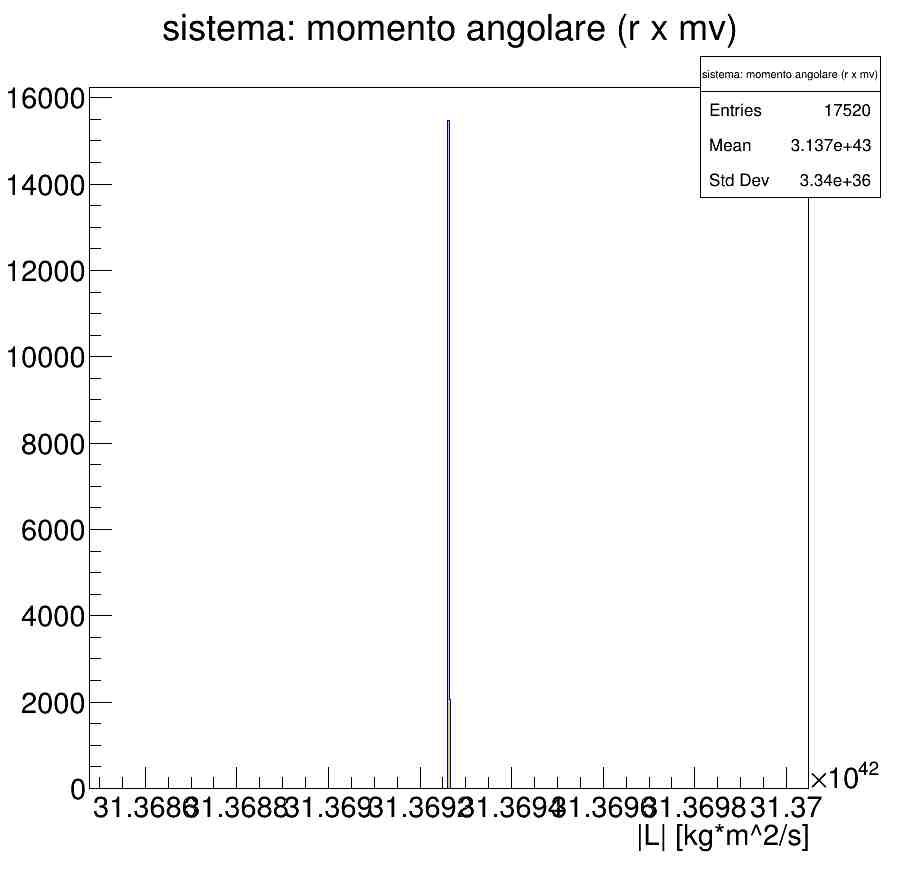
\includegraphics[width=4cm,height=3.5cm]{2_approx/L1_2.jpg}
                \label{cfr::L1}
                \column{.2\textwidth}
                \centering
                Metodo di Eulero\\
                \vspace{2cm}
                Eulero modificato
                \column{.4\textwidth}
                \centering
                %\caption{Orbita terrestre dopo 5 anni nei due metodi descritti}            
                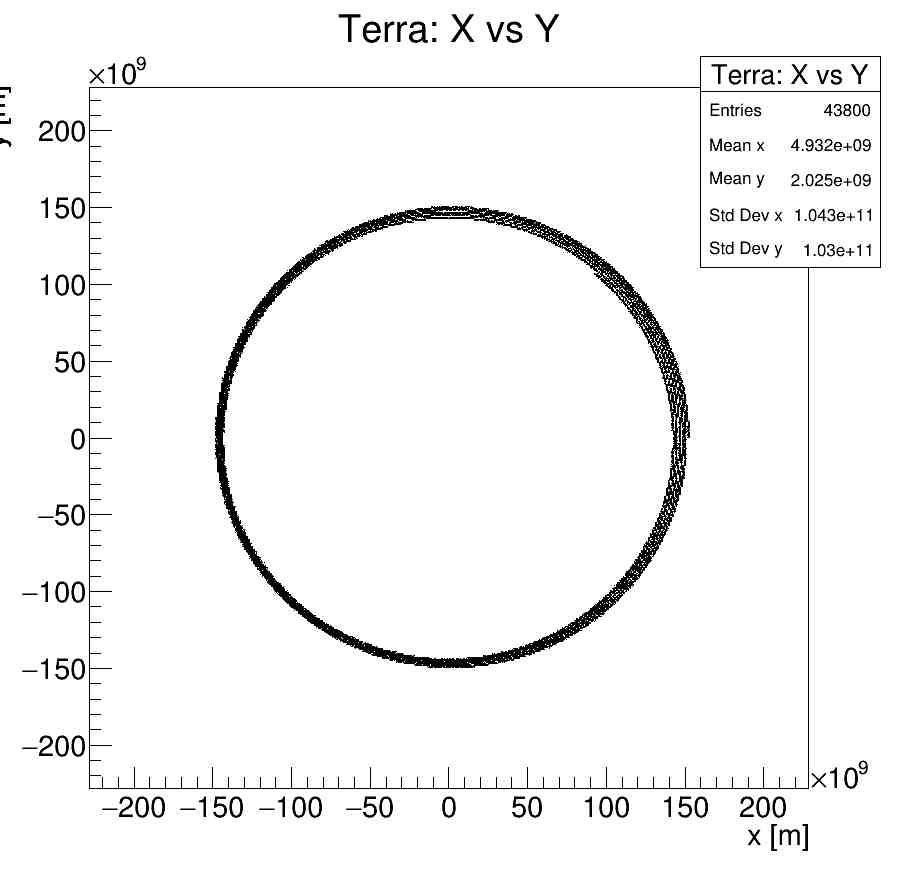
\includegraphics[width=3.75cm,height=3.75cm]{2_approx/terraxy_0_5.jpg}\\
                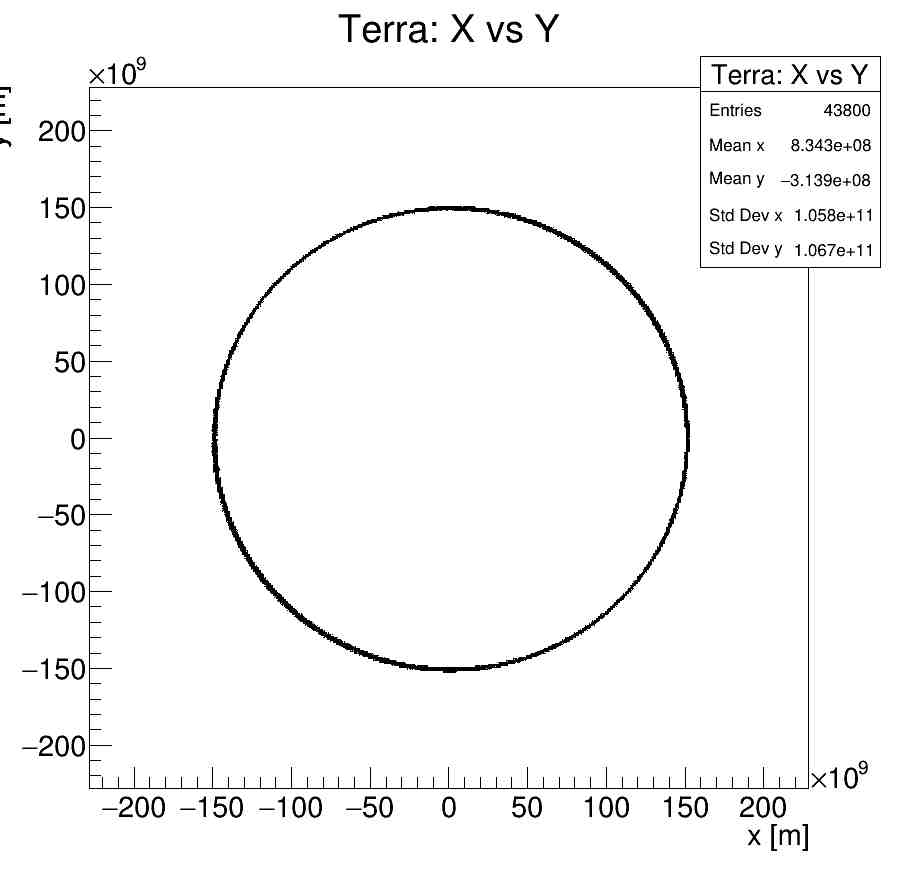
\includegraphics[width=3.75cm,height=3.75cm]{2_approx/terraxy_1_5.jpg}
                \label{cfr::xy1}
            \end{columns}
        \end{frame}
        
        \begin{frame}{deltaT=60s}
            \begin{columns}
                \column{.4\textwidth}
                    \centering
                    %\caption{Momento angolare del sistema dopo 100 anni nei due metodi descritti}            
                    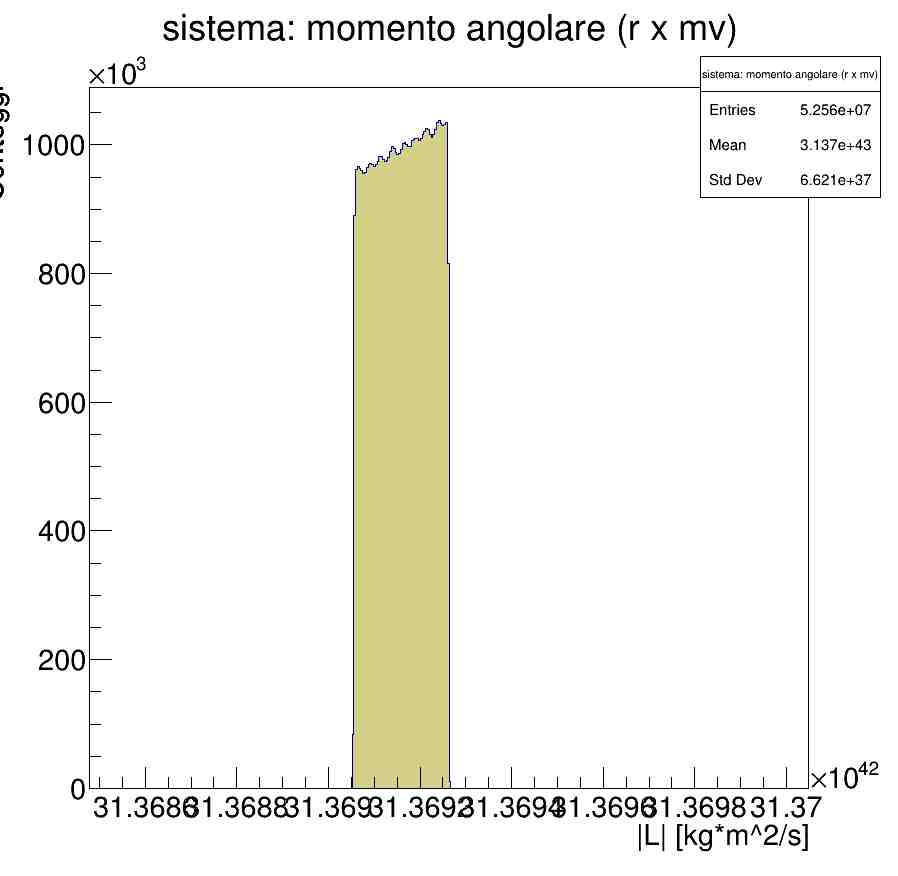
\includegraphics[width=4cm,height=4cm]{2_approx/L0_100.jpg}\\
                    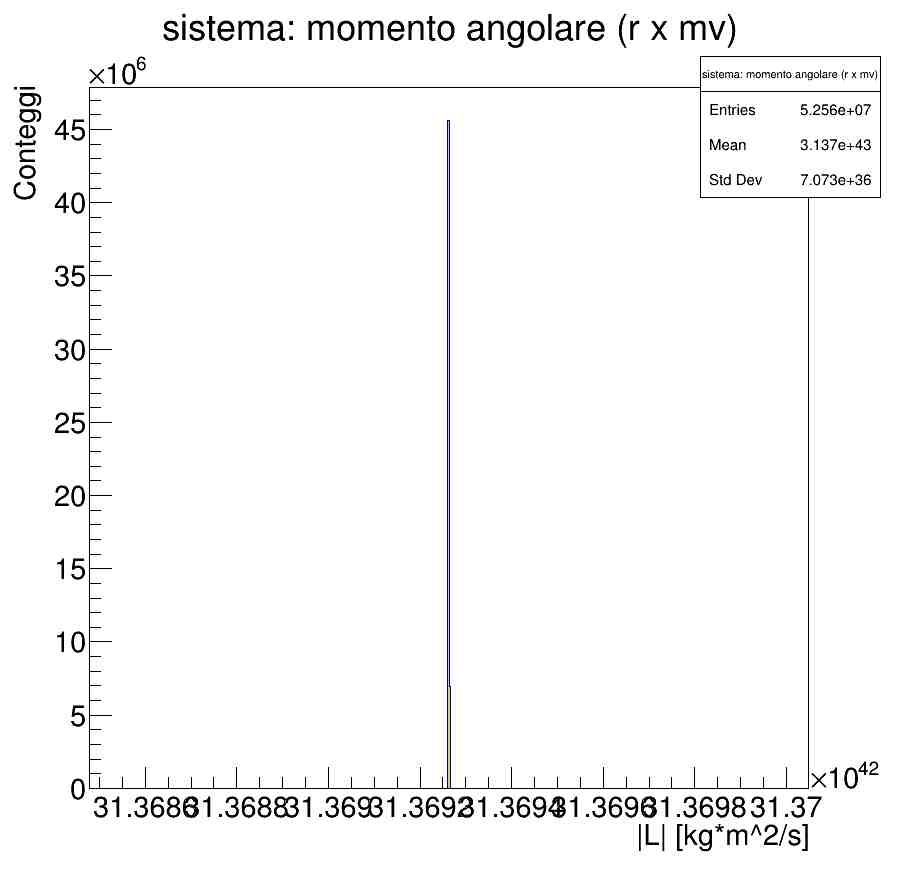
\includegraphics[width=4cm,height=3.5cm]{2_approx/L100_1.jpg}
                    \label{cfr::L2}
                \column{.2\textwidth}
                    \centering
                    Metodo di Eulero\\
                    \vspace{2cm}
                    Eulero modificato
                \column{.4\textwidth}
                    \centering
                    %\caption{Orbita terrestre dopo 100 anni nei due metodi descritti}            
                    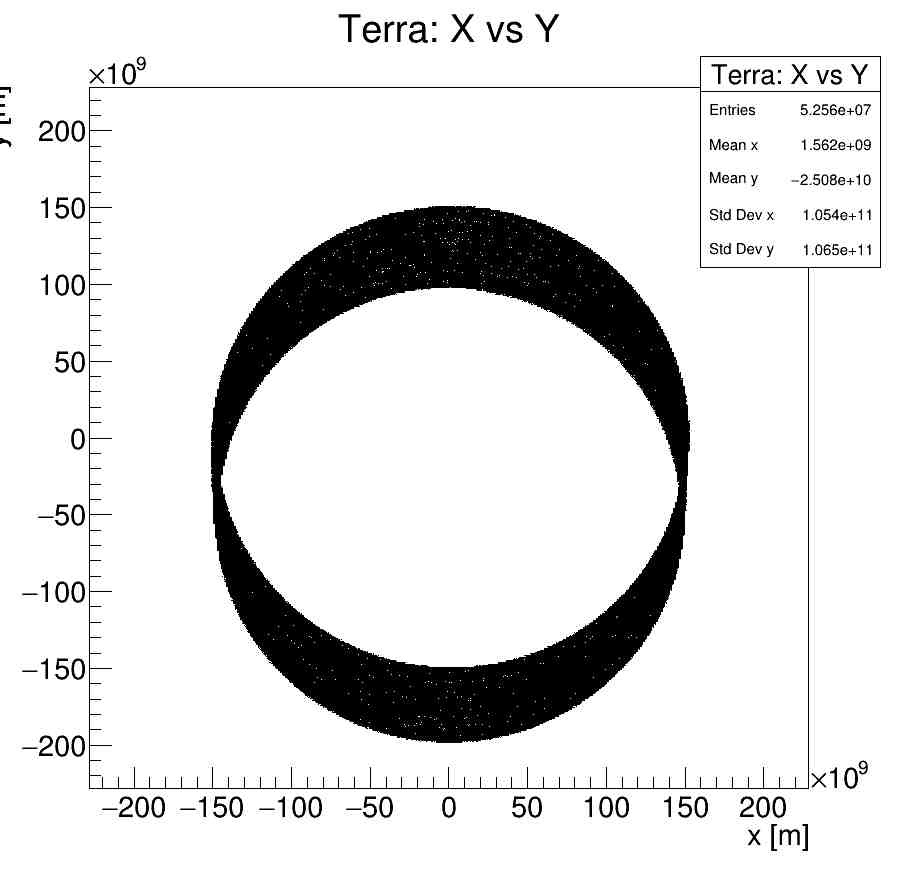
\includegraphics[width=3.75cm,height=3.75cm]{2_approx/terraxy_100_0.jpg}\\
                    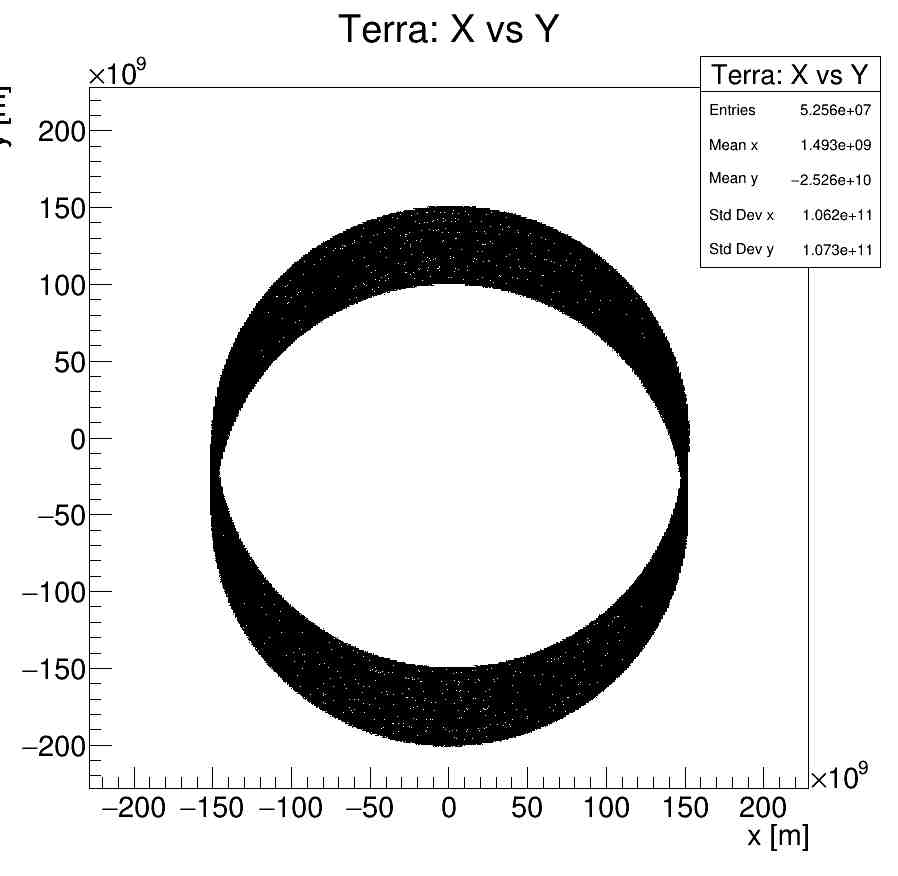
\includegraphics[width=3.75cm,height=3.75cm]{2_approx/terraxy_100__60_1.jpg}
                    \label{cfr::xy2}
            \end{columns}
        \end{frame}

        \begin{frame}{Altri Algoritmi}
            \begin{exampleblock}{$N>2 \Rightarrow$ Soluzione approssimata tramite metodi iterativi discreti:}
                \begin{enumerate}
                    \item Metodo di Eulero - approssimazione lineare
                    \item Runge-Kutta $2^{nd}$ order - Eulero modificato - limite 2000 anni
                    \item Runge-Kutta $2^{nd}$ order - altra versione
                    \item Velocity Verlet - sempre approssimazione del secondo ordine
                    \item Runge-Kutta $4^{th}$ - drifta subito ....
                    \item Yoshida $4^{th}$ order - algoritmo del quarto ordine - ma limiti come per velocity verlet ...
                \end{enumerate}
            \end{exampleblock}
            \begin{figure}
                \centering
                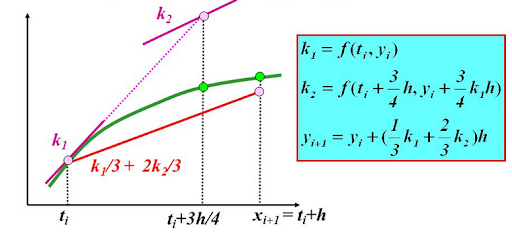
\includegraphics[width=0.5\linewidth]{2_approx/kutta.png}
                %\caption{Caption}
                \label{fig:kutt}
            \end{figure}
        \end{frame}

\section[Conserv]{Conservazione}
    \begin{frame}
        \frametitle{Contenuti}
        \transblindsvertical
        \tableofcontents[currentsection]
    \end{frame}

    \begin{frame}{Condizioni standarrd}
        \begin{alertblock}{La simulazione di riferimento con cui verranno fatti i vari confronti nelle slides successive è definita da:}
            \begin{enumerate}[a]
                \item Metodo di Eulero modificato - rapido e stabile per tempi medio-lunghi
                \item deltaT = 3600s - simulazioni rapide e stabili per tempi medio/lunghi
                \item T = 500 anni - durata media che permette già di notare patologie interessanti
                \item Configurazione iniziale mista - configurazione che dà risultati migliori, come vedremo in seguito
                \item Orbite tridimensionali
            \end{enumerate}
            Con queste cxondizioni una simulazione in C++ richiede circa 2min e 30s e circa 400MB(4\%) di memoria.\\
            Il tempo poi scala linearmente con il numero di step (determinate da T e deltaT).
        \end{alertblock}
    \end{frame}

    \begin{frame}{2D vs 3D}
        \begin{columns}
            \column{.5\textwidth}
                \centering
                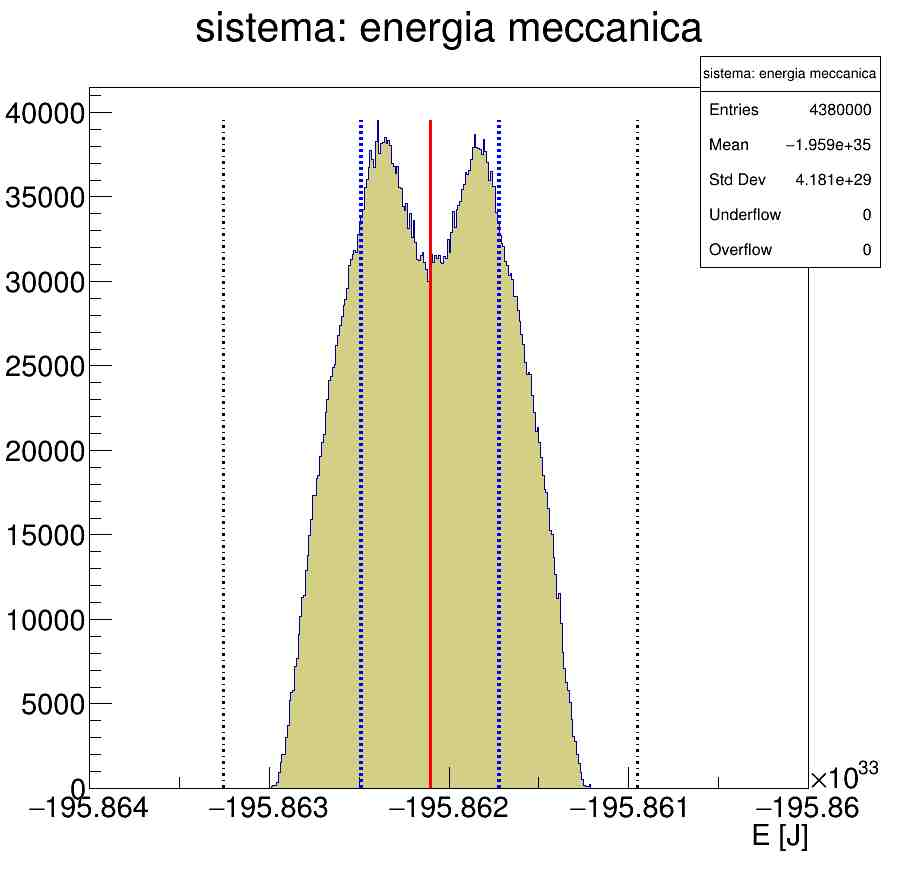
\includegraphics[width=5cm,height=3.75cm]{E2D.jpg}\\
                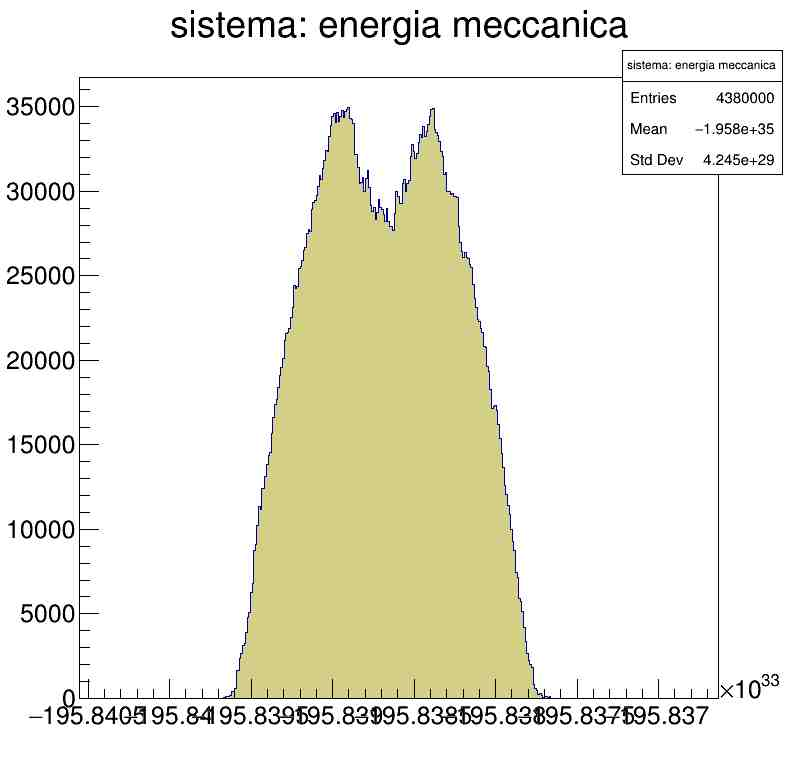
\includegraphics[width=5cm,height=3.75cm]{4_energia/E_500_3600.jpg}
                \label{cfr::E4T}              
            \column{.5\textwidth}
                \centering        
                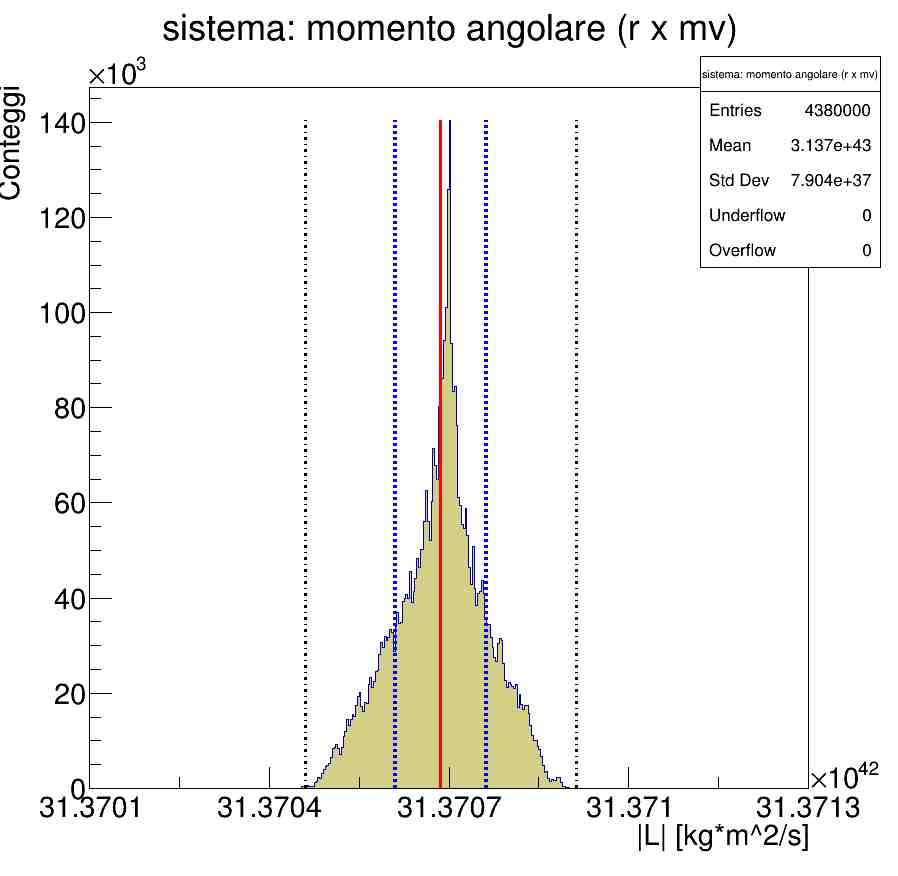
\includegraphics[width=5cm,height=3.75cm]{L2D.jpg}\\
                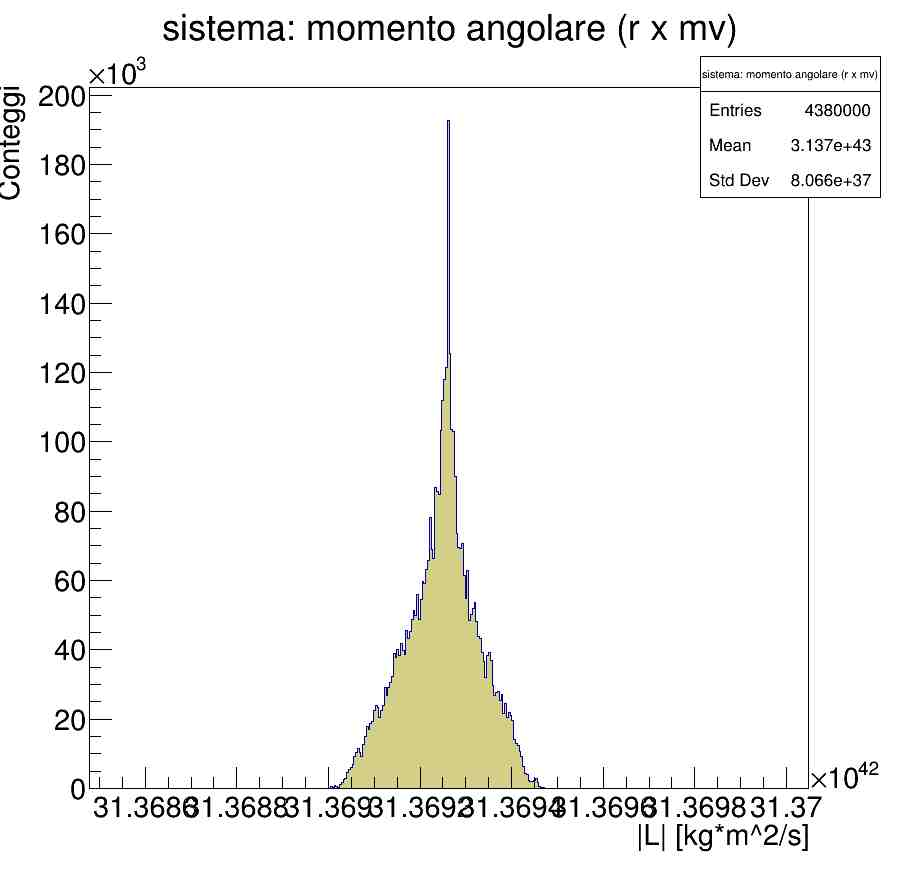
\includegraphics[width=5cm,height=3.75cm]{3_Momento/L_500_3600.jpg}
                \label{cfr::E6T}      
        \end{columns}
    \end{frame}

        \subsection[L]{Momento Angolare}
        \begin{frame}{L vs T | 100, 500, 2500 anni}
            \begin{columns}
                \column{.5\textwidth}
                    \centering        
                    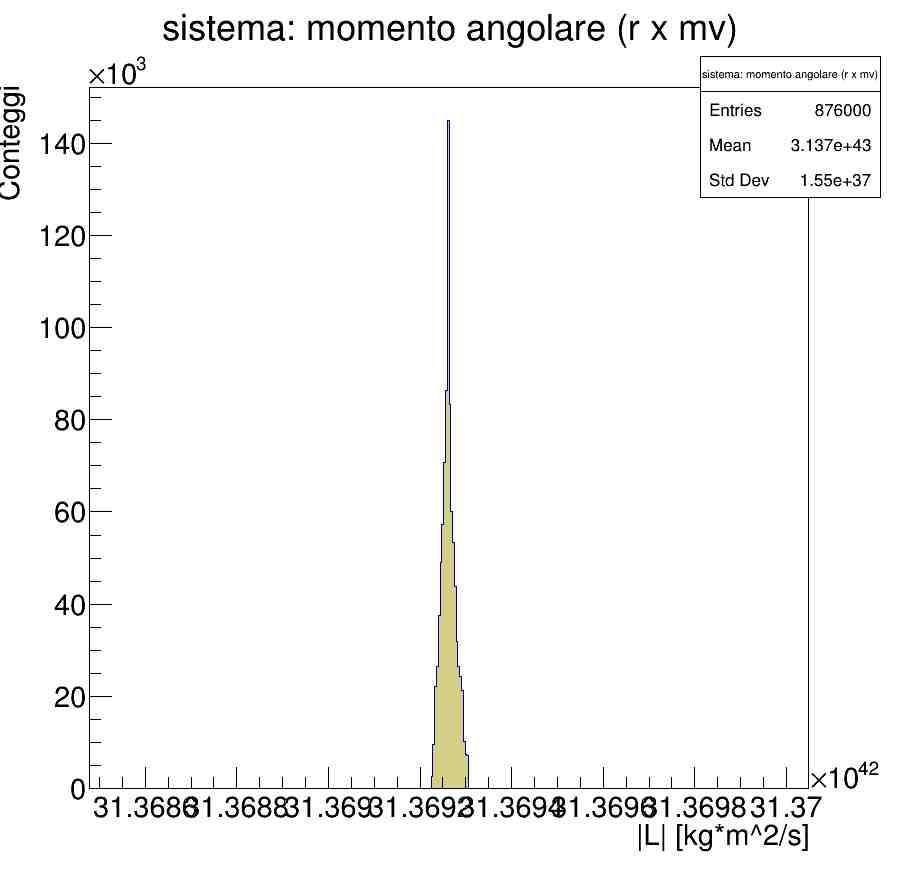
\includegraphics[width=5cm,height=3.75cm]{3_Momento/L_100_3600.jpg}\\
                    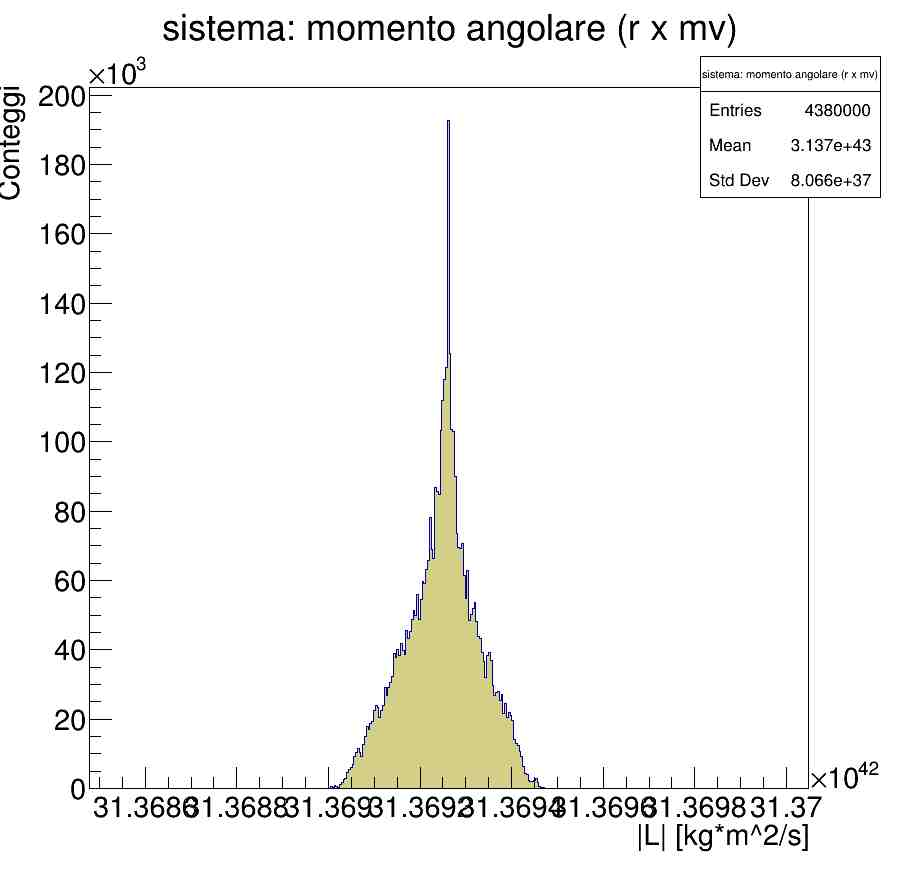
\includegraphics[width=5cm,height=3.75cm]{3_Momento/L_500_3600.jpg}
                    \label{cfr::LT}              
                \column{.5\textwidth}
                    \centering        
                    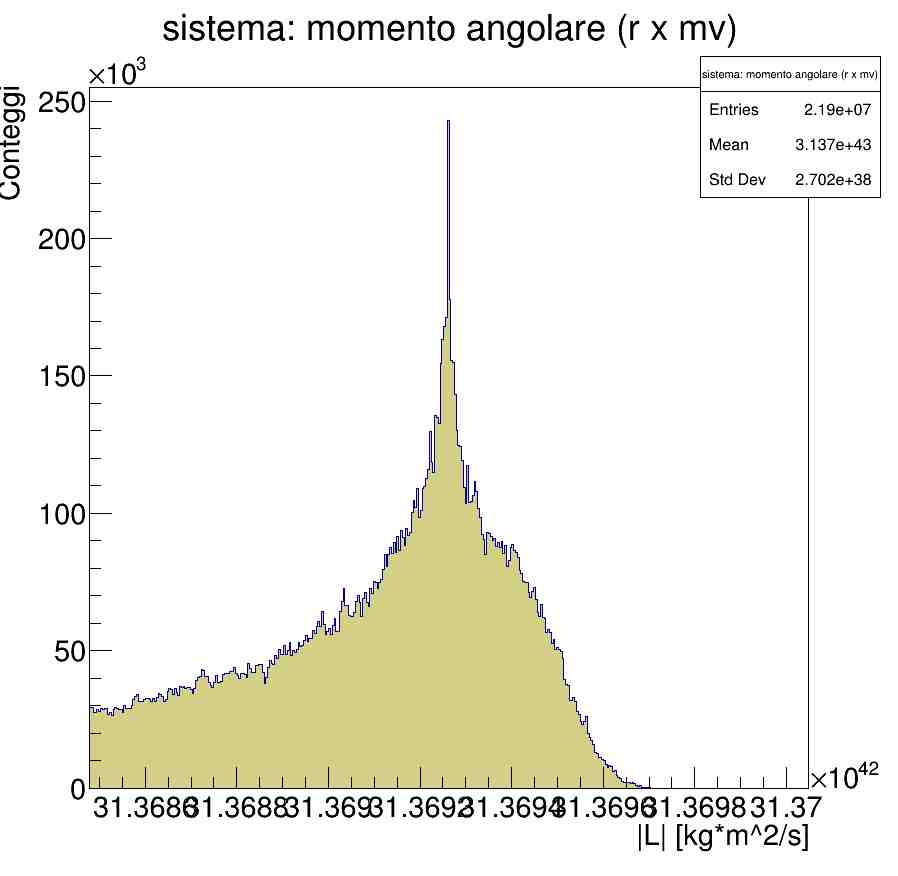
\includegraphics[width=5cm,height=3.75cm]{3_Momento/L_2500_3600_stretto.jpg}\\
                    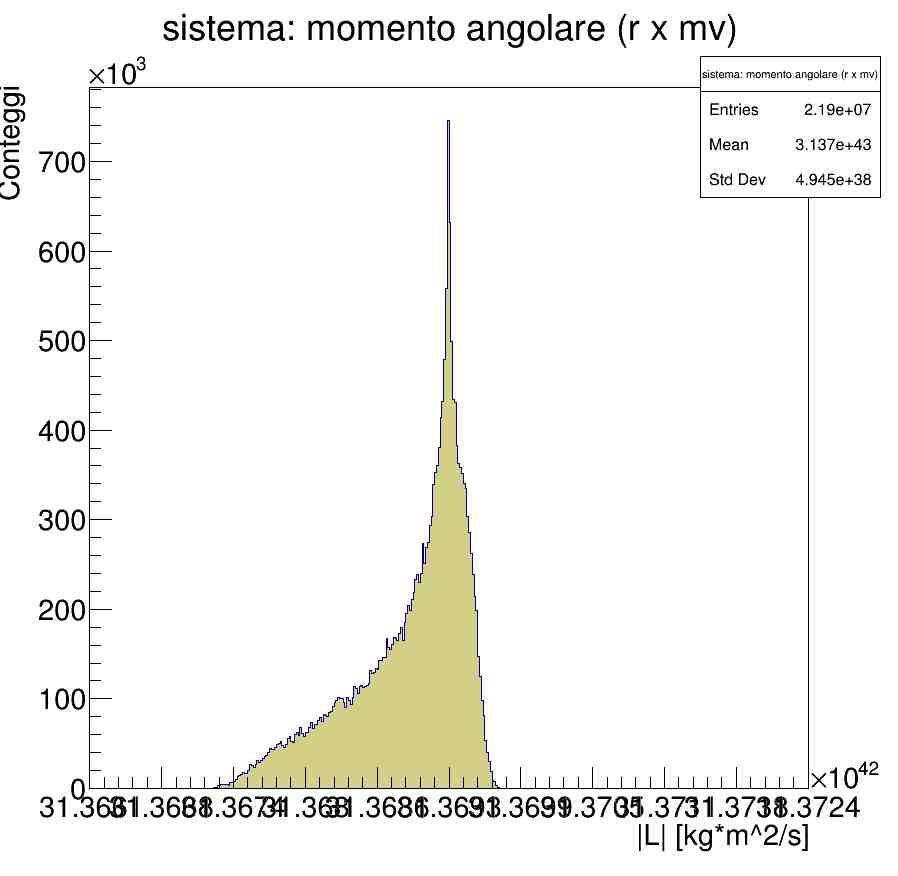
\includegraphics[width=5cm,height=3.75cm]{3_Momento/L_2500_3600_larg.jpg}
                    \label{cfr::LT2}      
            \end{columns}
        \end{frame}
        
        \begin{frame}{L vs deltaT | 60, 1800, 3600 secondi}
            \begin{columns}
                \column{.5\textwidth}
                    \centering        
                    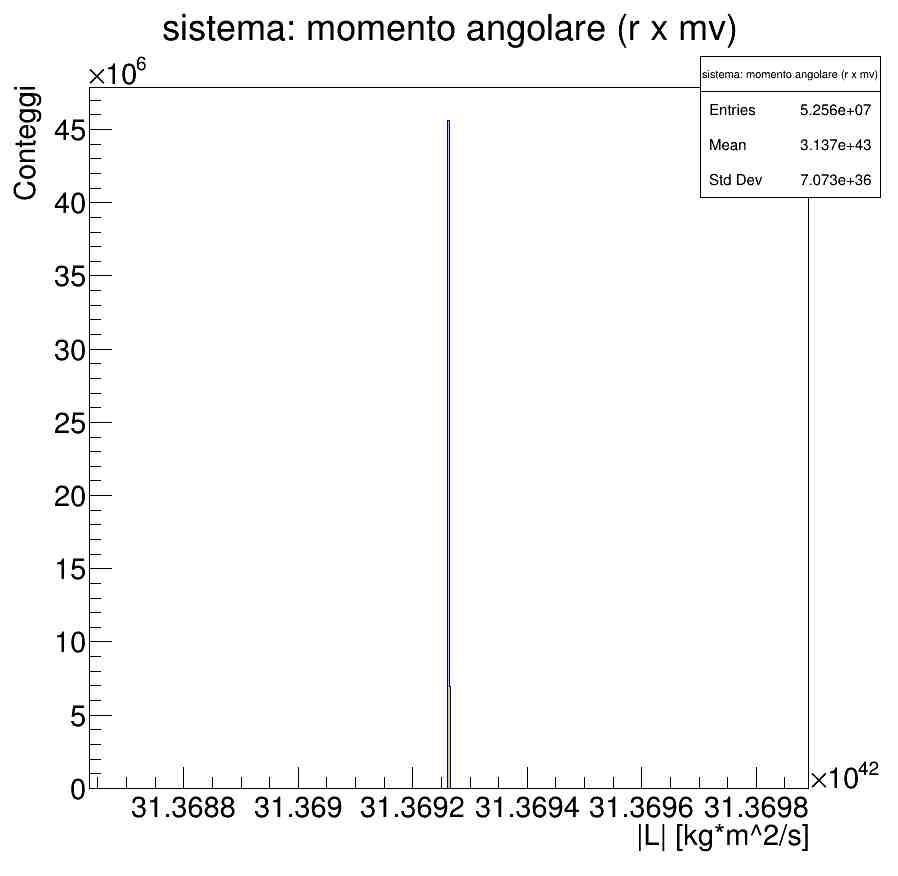
\includegraphics[width=5cm,height=3.75cm]{3_Momento/L_100_60.jpg}\\
                    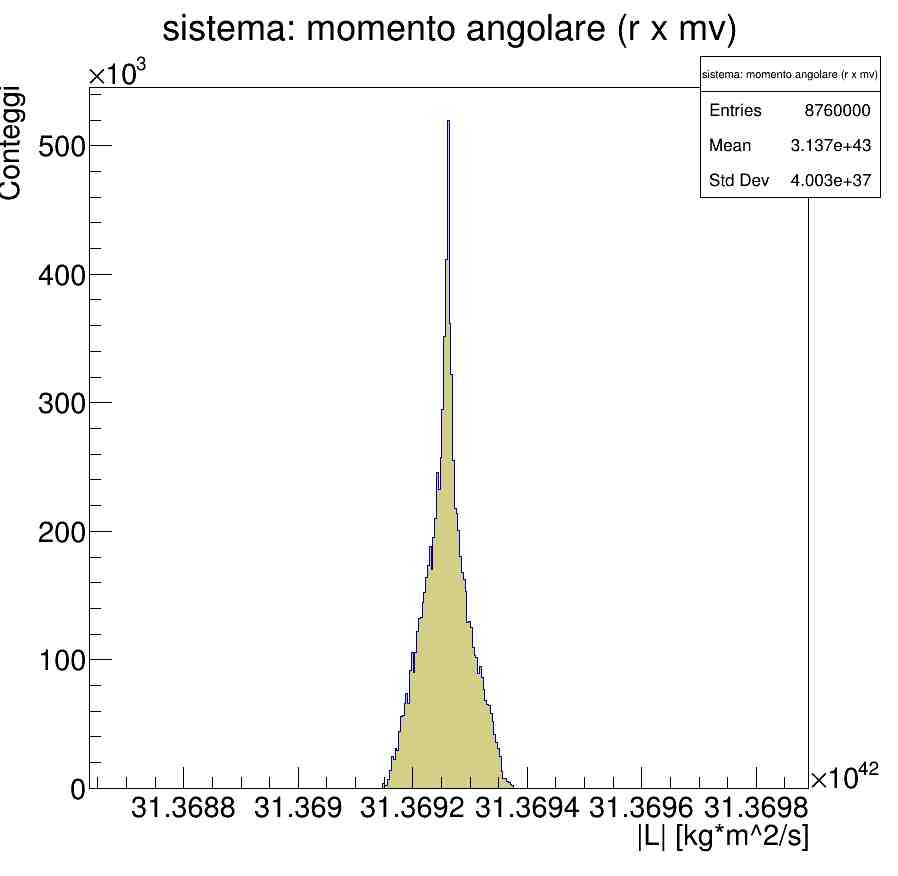
\includegraphics[width=5cm,height=3.75cm]{3_Momento/L_500_1800.jpg}
                    \label{cfr::LT3}              
                \column{.5\textwidth}
                    \centering        
                    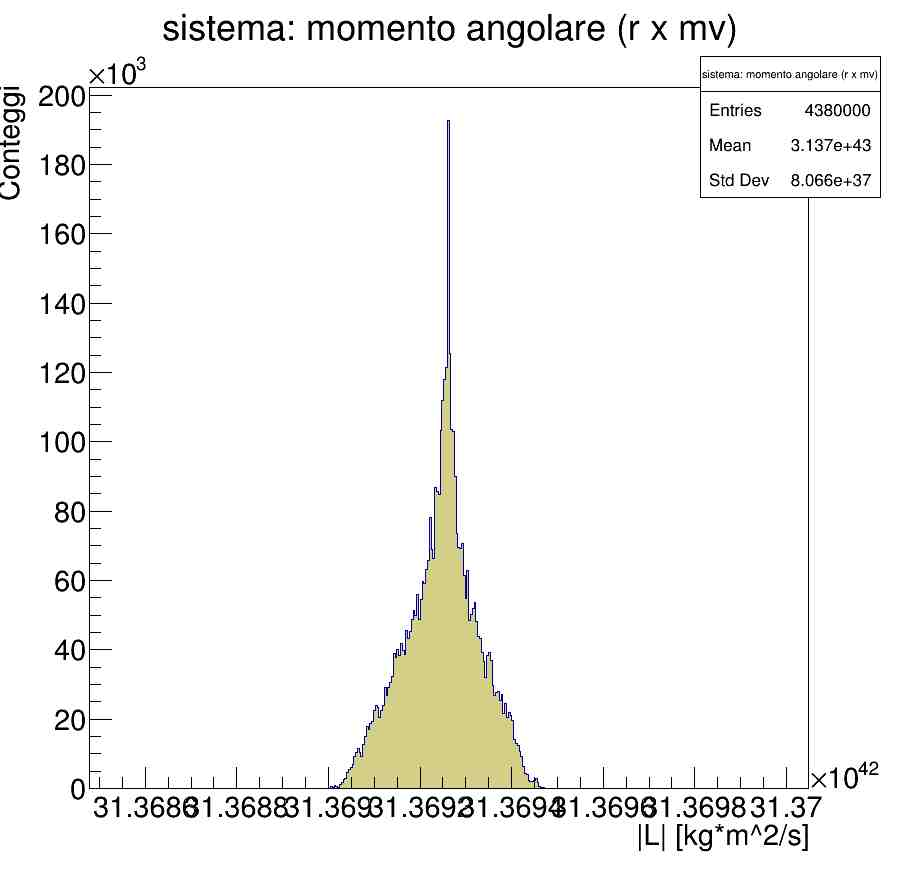
\includegraphics[width=5cm,height=3.75cm]{3_Momento/L_500_3600.jpg}\\
                    \label{cfr::LT4}
                    Istogrammi più piccati, ma in generale Media simile e DevStd dello stesso ordine - per notare differenze importanti si dovrebbe aumentare molto anche T, ma la simulazione sarebbe troppo lunga
            \end{columns}            
        \end{frame}
        
        \begin{frame}{L vs posizioni iniziali | perielio, afelio, medie, miste}
            \begin{columns}
                \column{.5\textwidth}
                    \centering        
                    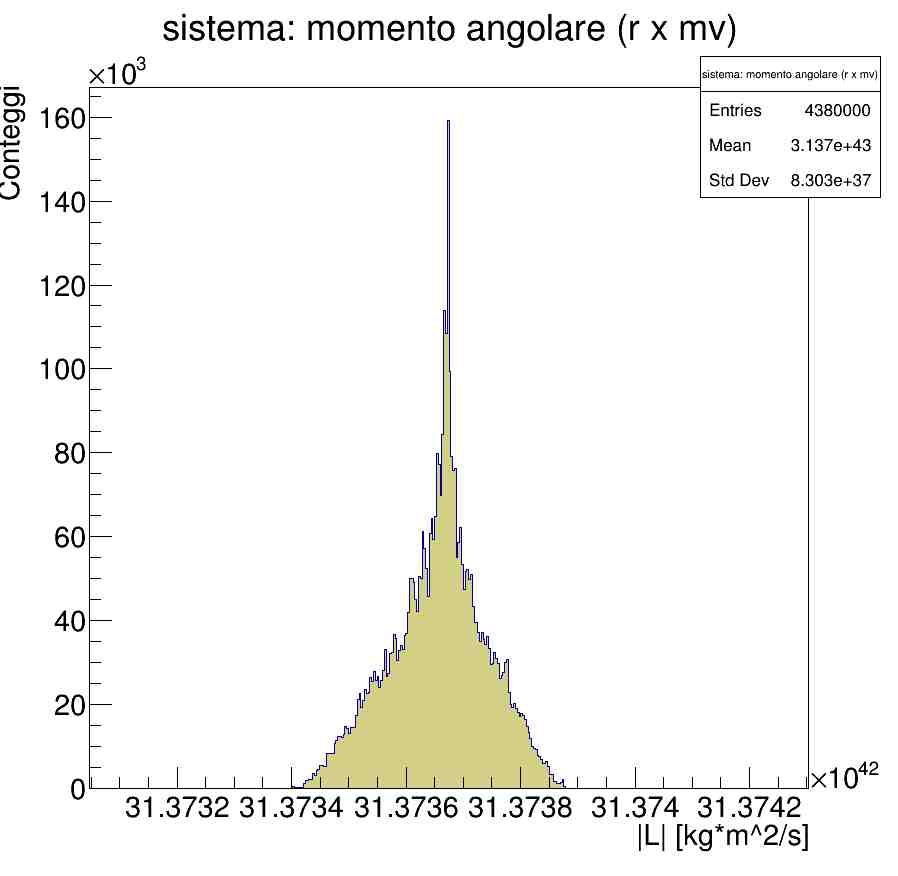
\includegraphics[width=5cm,height=3.75cm]{3_Momento/L_500_peri.jpg}\\
                    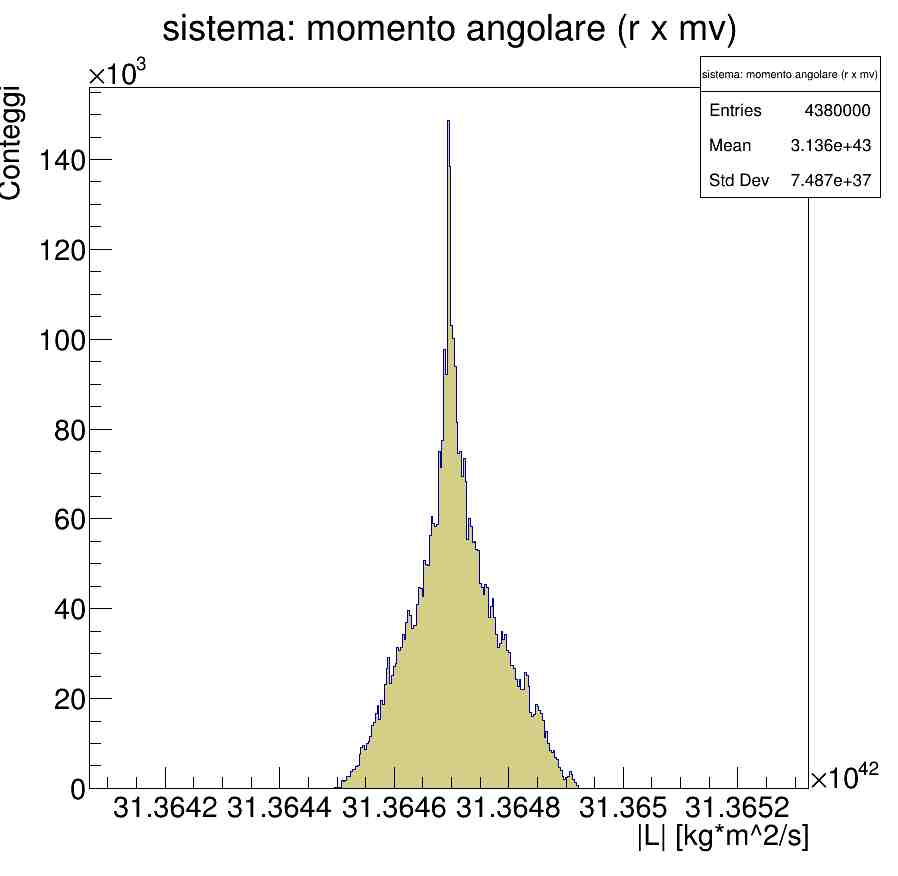
\includegraphics[width=5cm,height=3.75cm]{3_Momento/L_500_afe.jpg}
                    \label{cfr::LT5}              
                \column{.5\textwidth}
                    \centering        
                    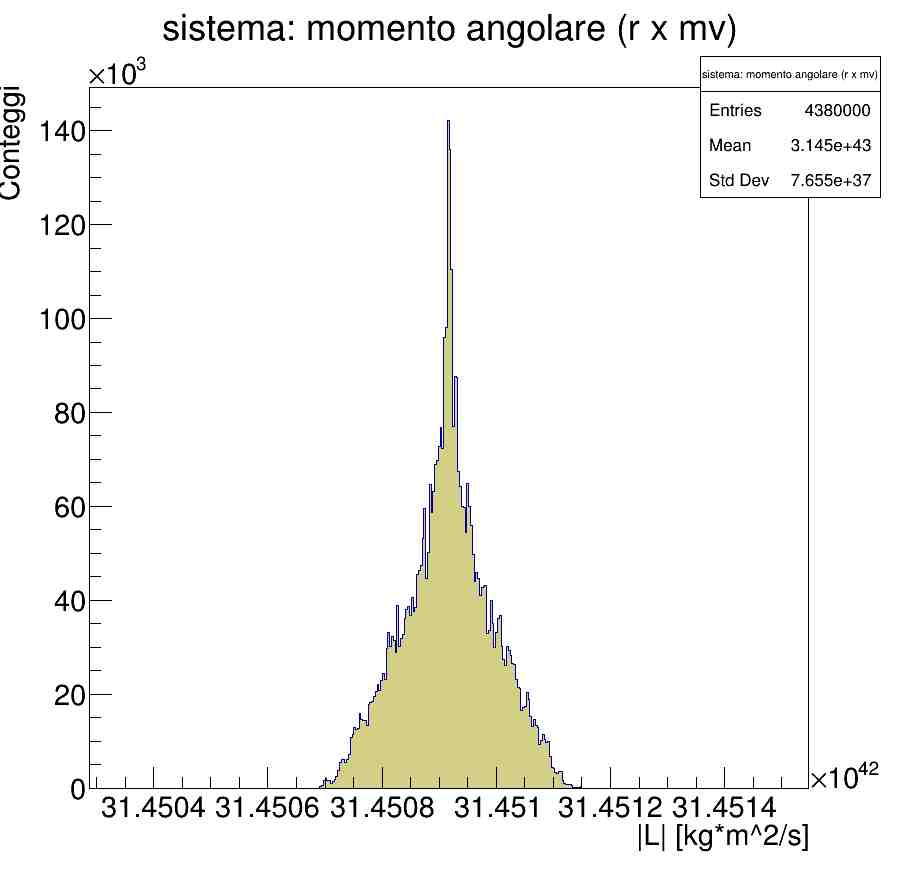
\includegraphics[width=5cm,height=3.75cm]{3_Momento/L_500_medi.jpg}\\
                    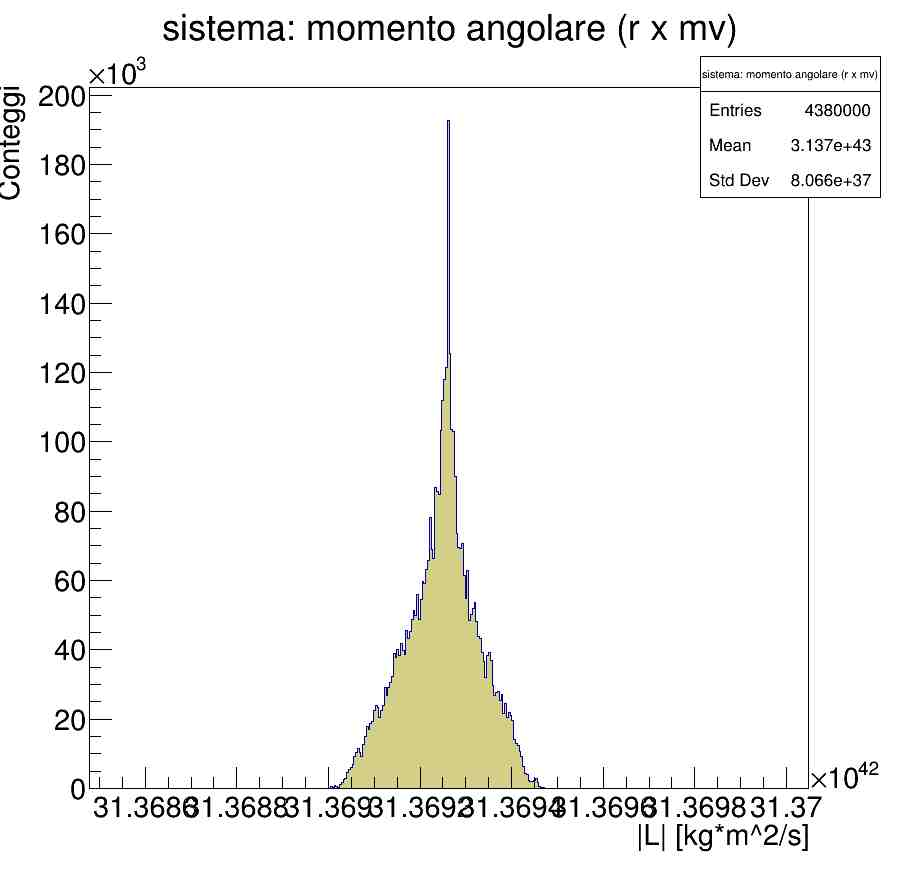
\includegraphics[width=5cm,height=3.75cm]{3_Momento/L_500_3600.jpg}
                    \label{cfr::LT6}      
            \end{columns}
        \end{frame}
    
    \subsection[E]{Energia Meccanica}
        \begin{frame}{E vs T | 100, 500, 2500 anni}
            \begin{columns}
                \column{.5\textwidth}
                    \centering        
                    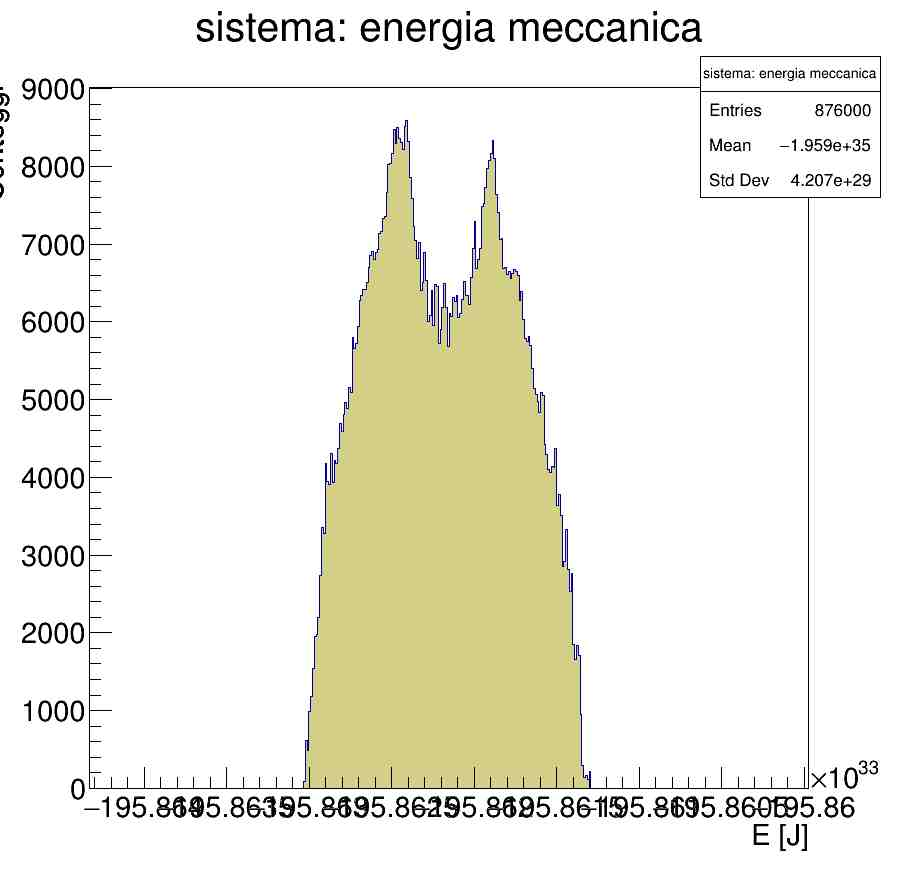
\includegraphics[width=5cm,height=3.75cm]{4_energia/E_100_3600.jpg}\\
                    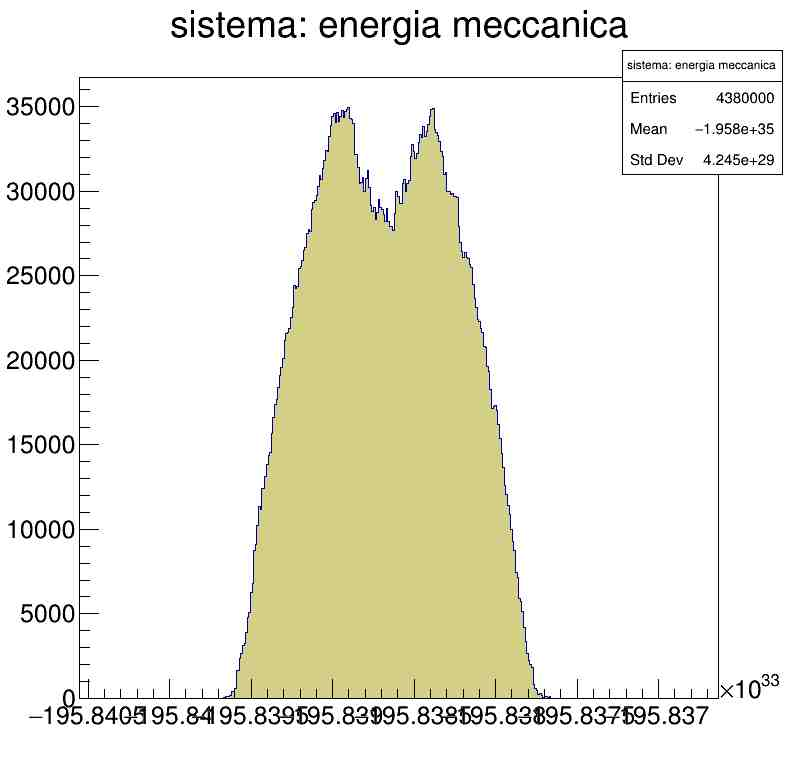
\includegraphics[width=5cm,height=3.75cm]{4_energia/E_500_3600.jpg}
                    \label{cfr::ET}              
                \column{.5\textwidth}
                    \centering        
                    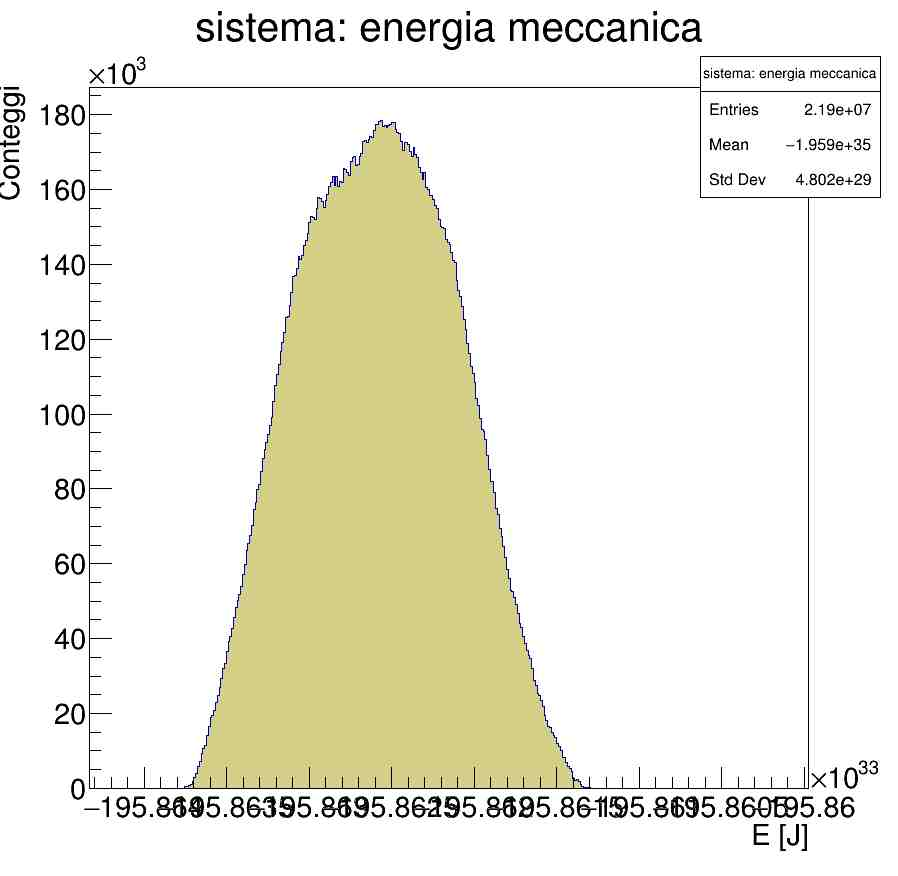
\includegraphics[width=5cm,height=3.75cm]{4_energia/E_2500_3600_stretto.jpg}\\
                    \label{cfr::ET1}
                    Media vicina - leggero aumento della DevStd col tempo
            \end{columns}
        \end{frame}
        \begin{frame}{E vs deltaT | 60, 1800, 3600 secondi}
            \begin{columns}
                \column{.5\textwidth}
                    \centering        
                    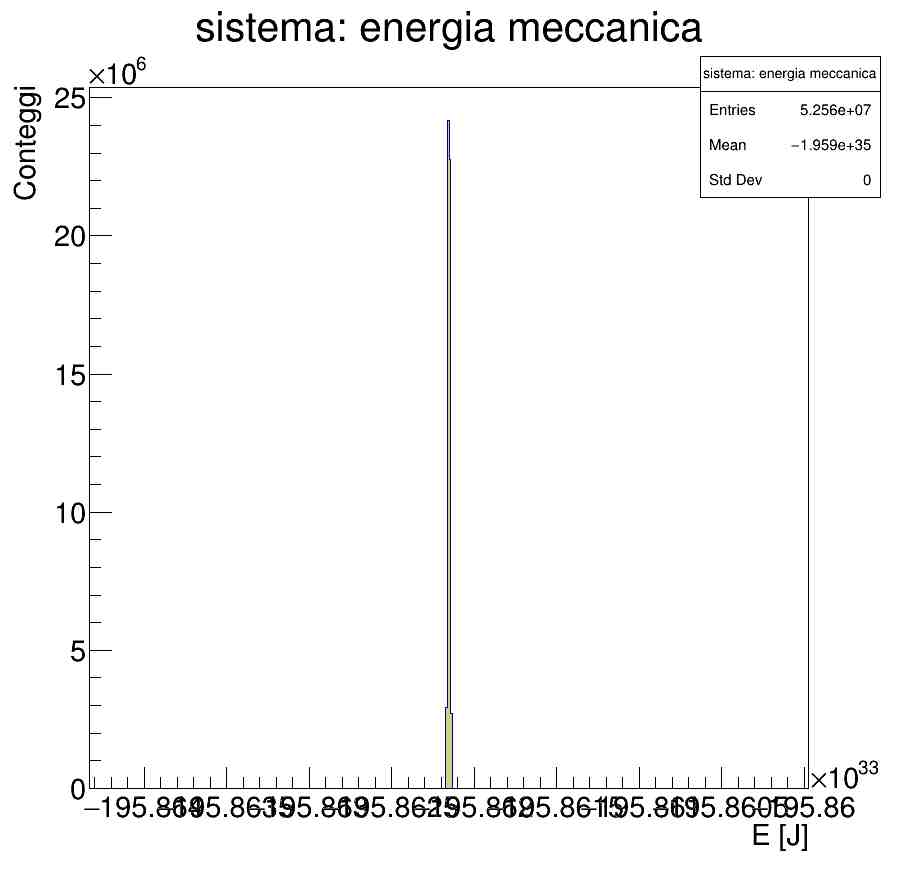
\includegraphics[width=5cm,height=3.75cm]{4_energia/E_100_60.jpg}\\
                    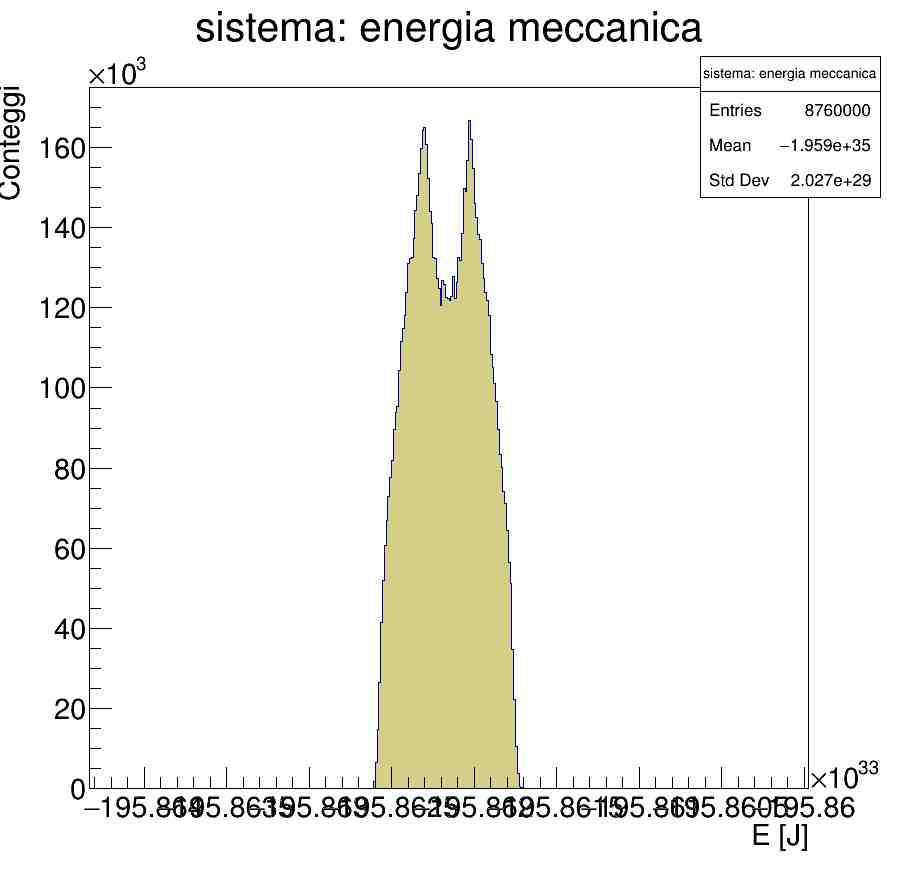
\includegraphics[width=5cm,height=3.75cm]{4_energia/E_500_1800.jpg}
                    \label{cfr::E3}              
                \column{.5\textwidth}
                    \centering        
                    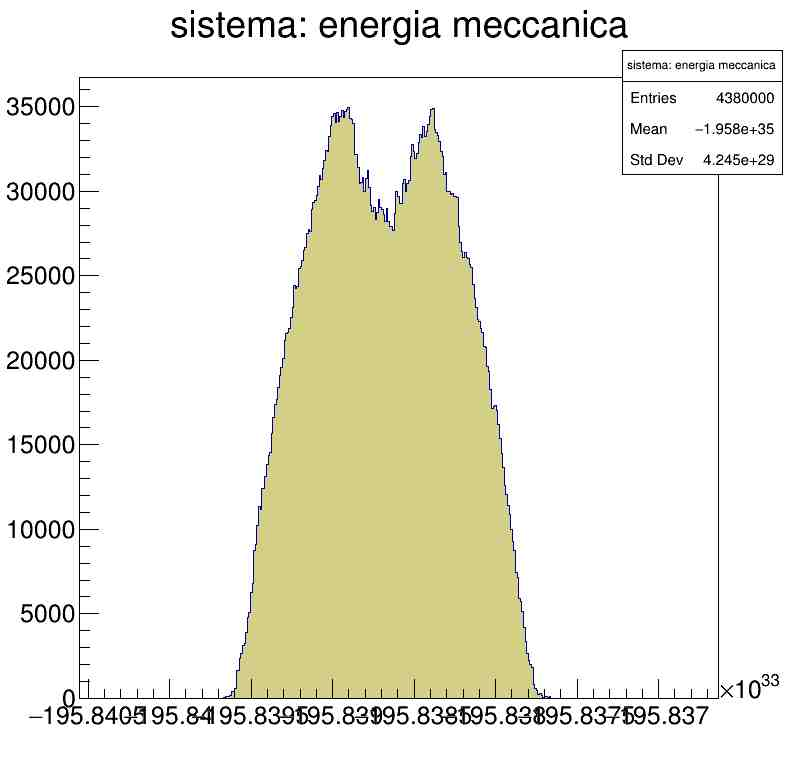
\includegraphics[width=5cm,height=3.75cm]{4_energia/E_500_3600.jpg}\\
                    \label{cfr::E2T}
                    Si nota molto di più l'effetto rispetto agli istogrammi di L
            \end{columns}            
        \end{frame}
        \begin{frame}{E vs posizioni iniziali | perielio, afelio, medie, miste}
            \begin{columns}
                \column{.5\textwidth}
                    \centering        
                    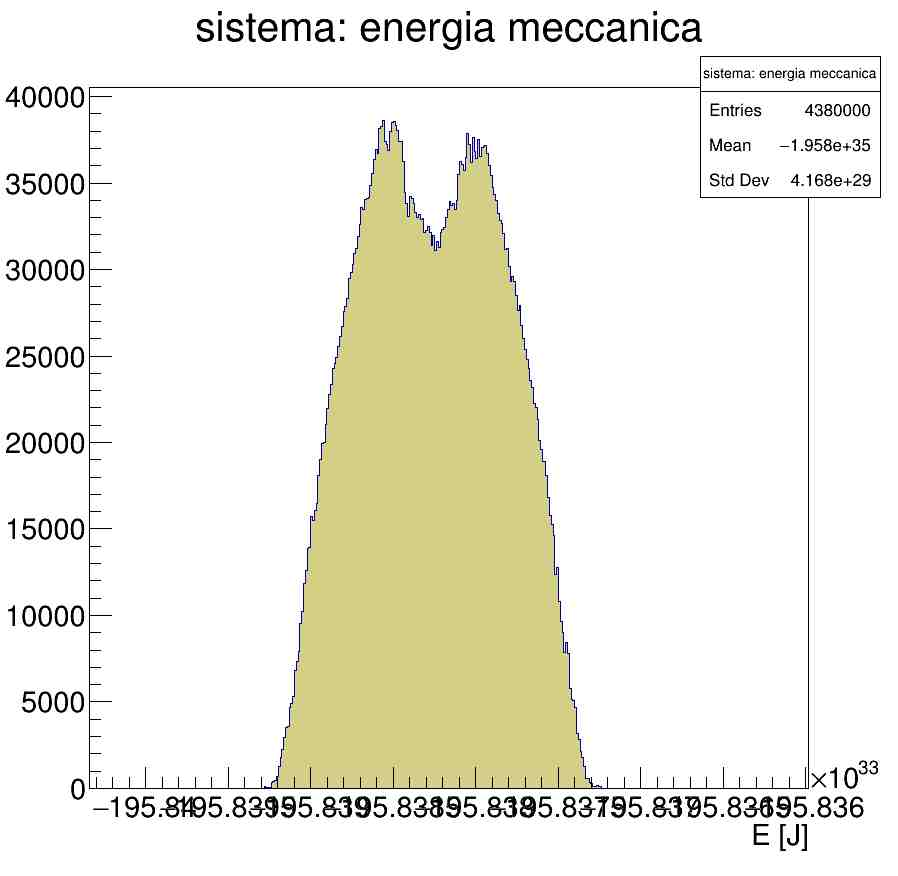
\includegraphics[width=5cm,height=3.75cm]{4_energia/E_500_peri.jpg}\\
                    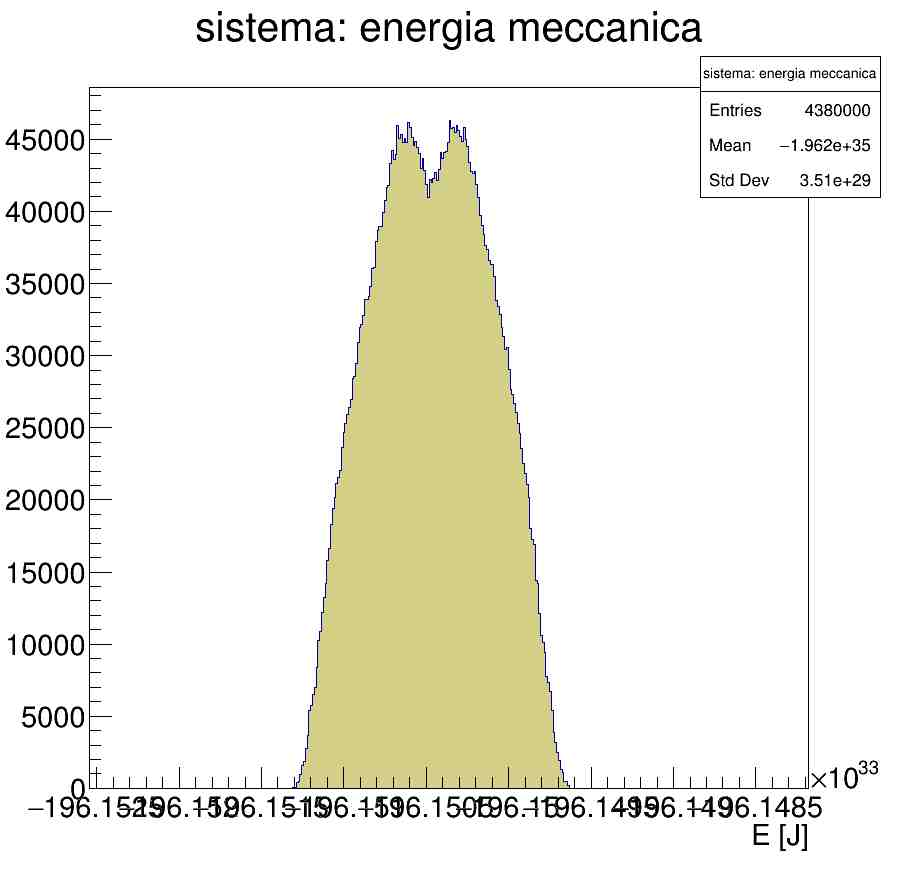
\includegraphics[width=5cm,height=3.75cm]{4_energia/E_500_afe.jpg}
                    \label{cfr::E4T}              
                \column{.5\textwidth}
                    \centering        
                    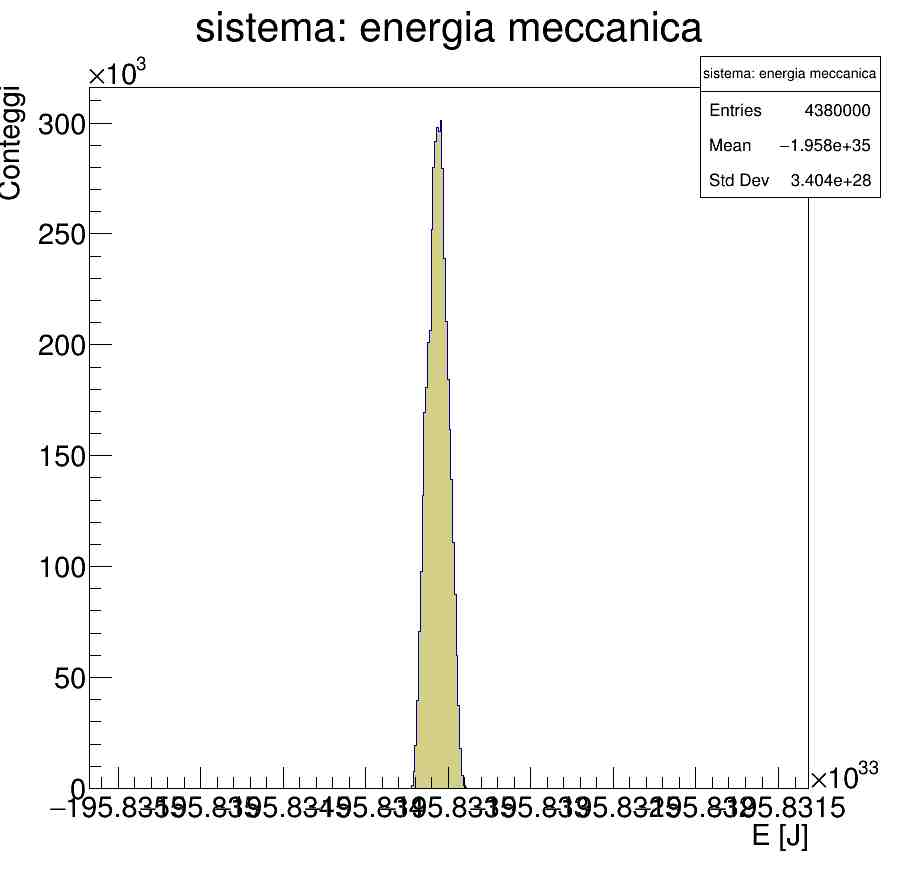
\includegraphics[width=5cm,height=3.75cm]{4_energia/E_500_medi.jpg}\\
                    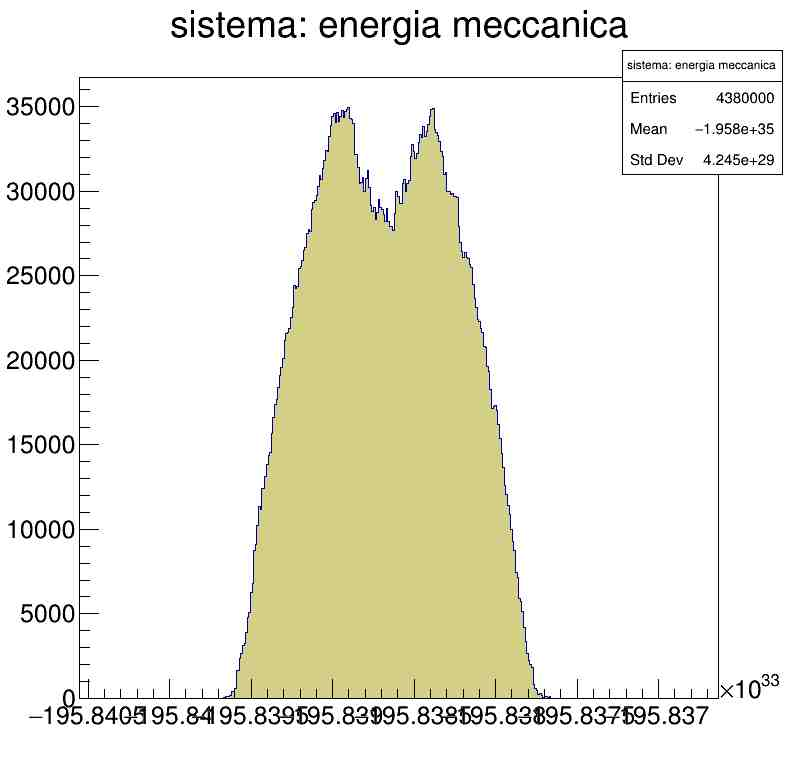
\includegraphics[width=5cm,height=3.75cm]{4_energia/E_500_3600.jpg}
                    \label{cfr::E6T}      
            \end{columns}
        \end{frame}

        \begin{frame}{Istogramma con Python}
            \begin{figure}
                \centering
                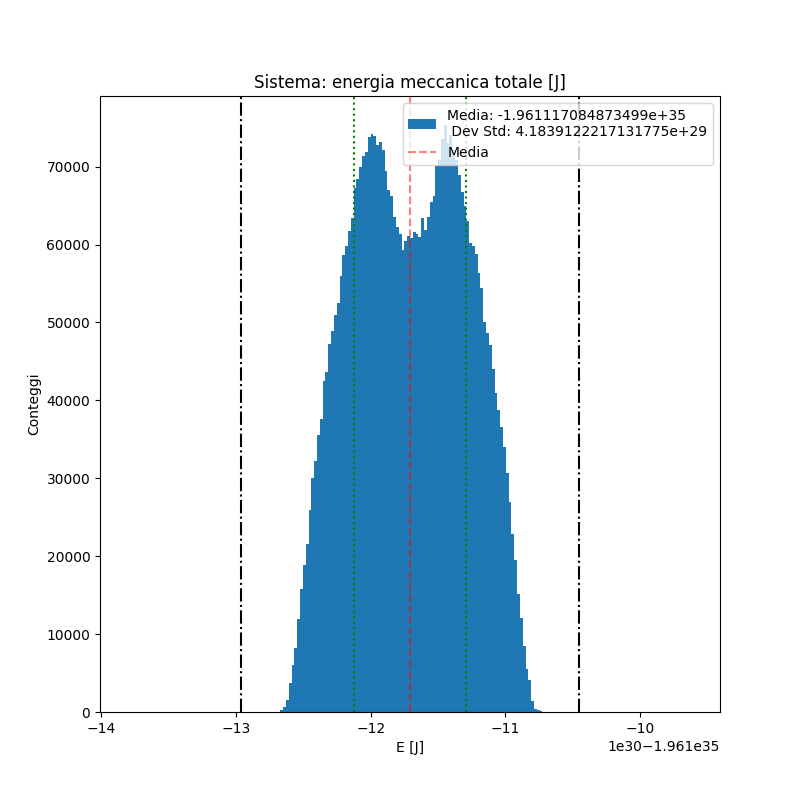
\includegraphics[height=8cm]{4_energia/E_500_3600_py-.png}
                %\caption{Caption}
                %\label{fig:enter-label}
            \end{figure}
        \end{frame}

        \subsubsection[DP]{Double Peak}
                    \begin{frame}{Studio del doppio picco}
            \begin{columns}
                \column{.5\textwidth}
                    \centering        
                    \includegraphics[width=5cm,height=3.75cm]{4_energia/peak/}\\
                    %quì cinetica vs Pot
                    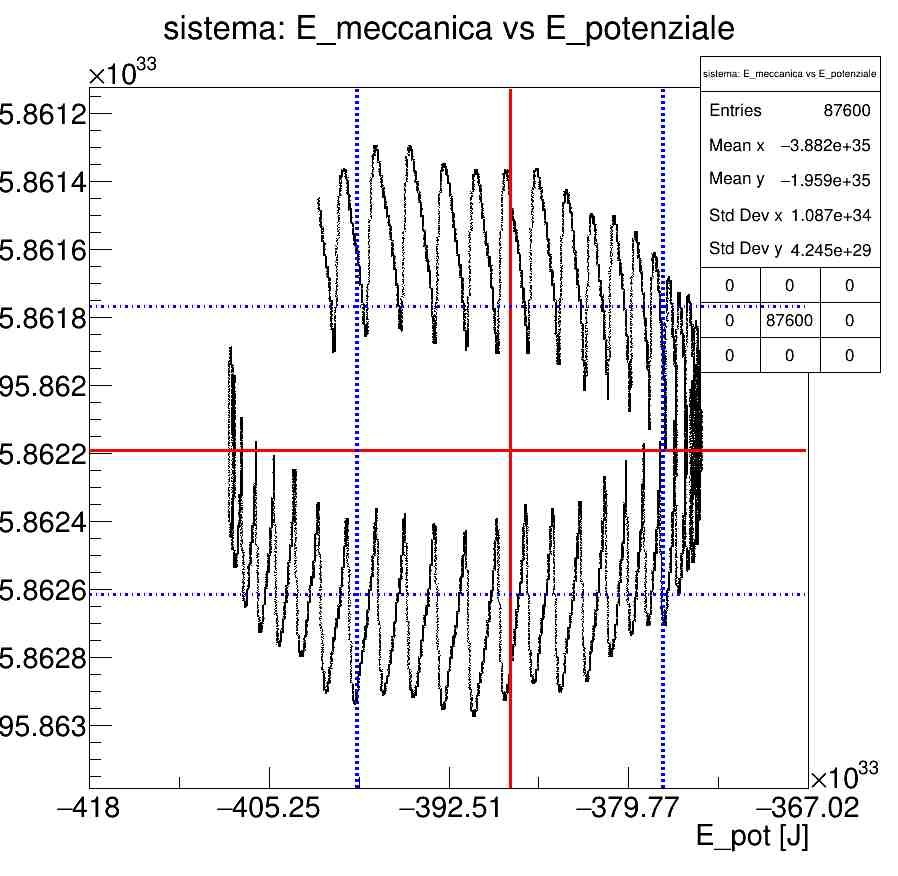
\includegraphics[width=5cm,height=3.75cm]{4_energia/peak/Mec_pot.jpg}
                    \label{cfr::Epc}              
                \column{.5\textwidth}
                    \centering        
                    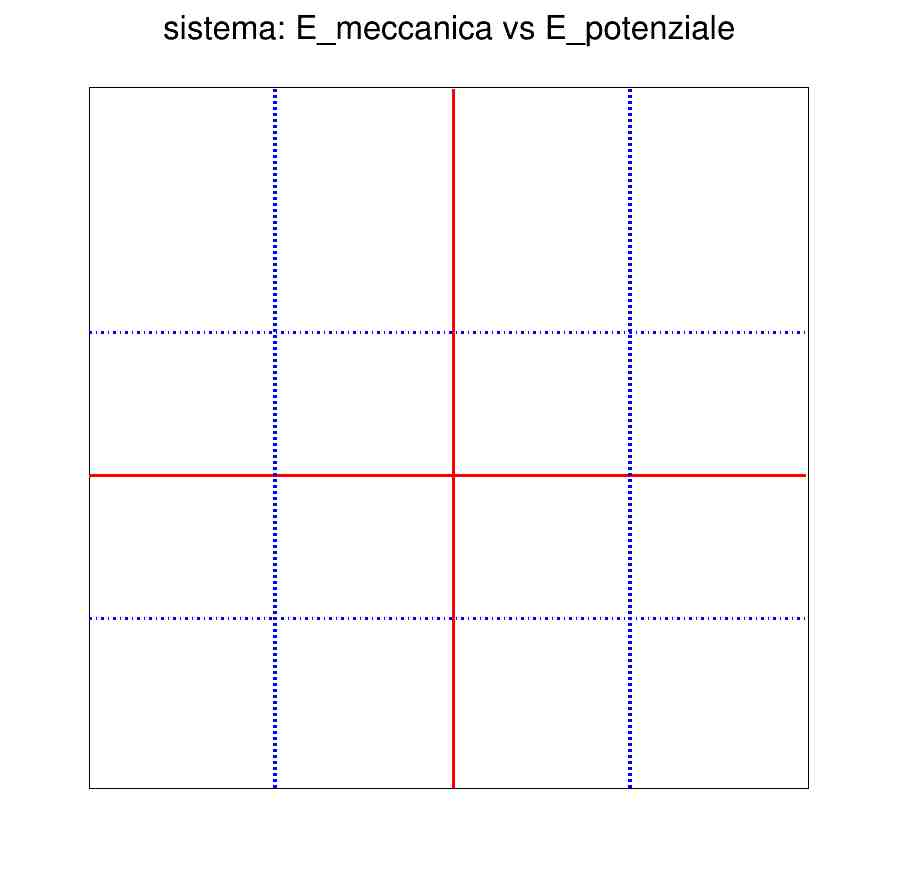
\includegraphics[width=5cm,height=3.75cm]{4_energia/peak/m_p_500.jpg}\\
                    %qui grafico E vs Pot dopo 500a
                    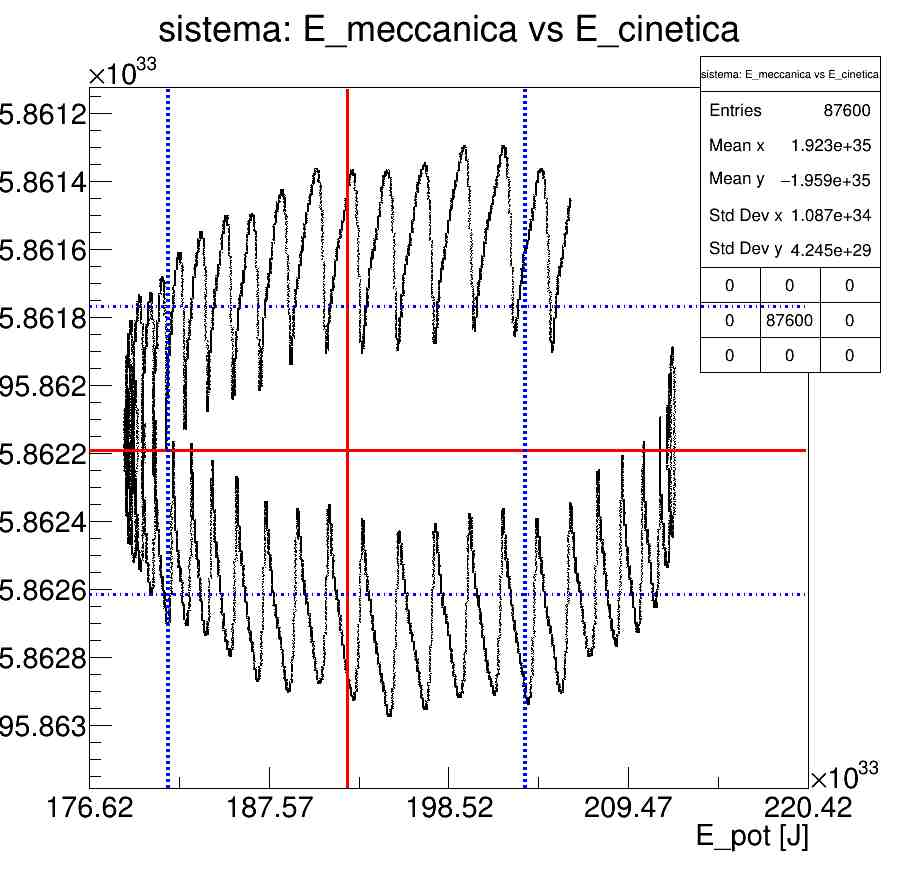
\includegraphics[width=5cm,height=3.75cm]{4_energia/peak/mec_cin.jpg}
                    \label{cfr::eme}      
            \end{columns}
        \end{frame}
        \begin{frame}{Studio del doppio picco}
            \begin{columns}
                \column{.5\textwidth}
                    \centering        
                    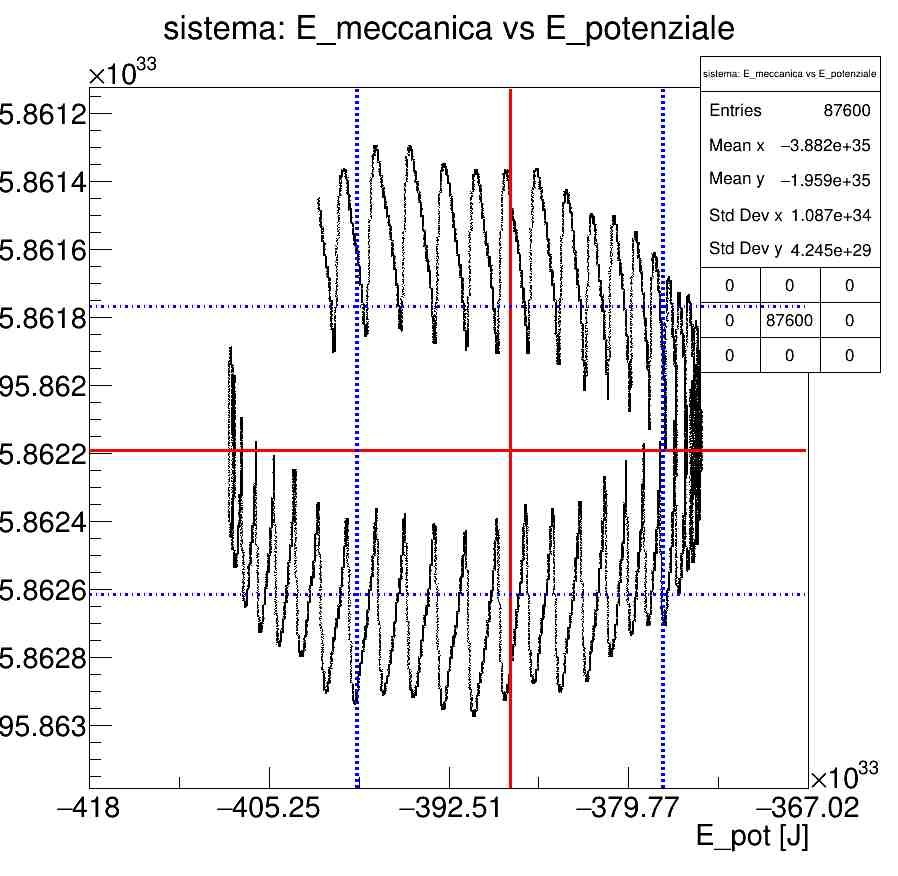
\includegraphics[width=5cm,height=3.75cm]{4_energia/peak/Mec_pot.jpg}\\
                    \label{cfr::E4T}              
                \column{.5\textwidth}
                    \centering        
                    \includegraphics[width=5cm,height=3.75cm]{4_energia/peak/mec_gio.jpg}\\
                    %qui grafico E vs dgiove-sole
                    \label{cfr::E6T}      
            \end{columns}
        \end{frame}

        \begin{frame}{Andamenti nel tempo}
            \begin{figure}
                \centering
                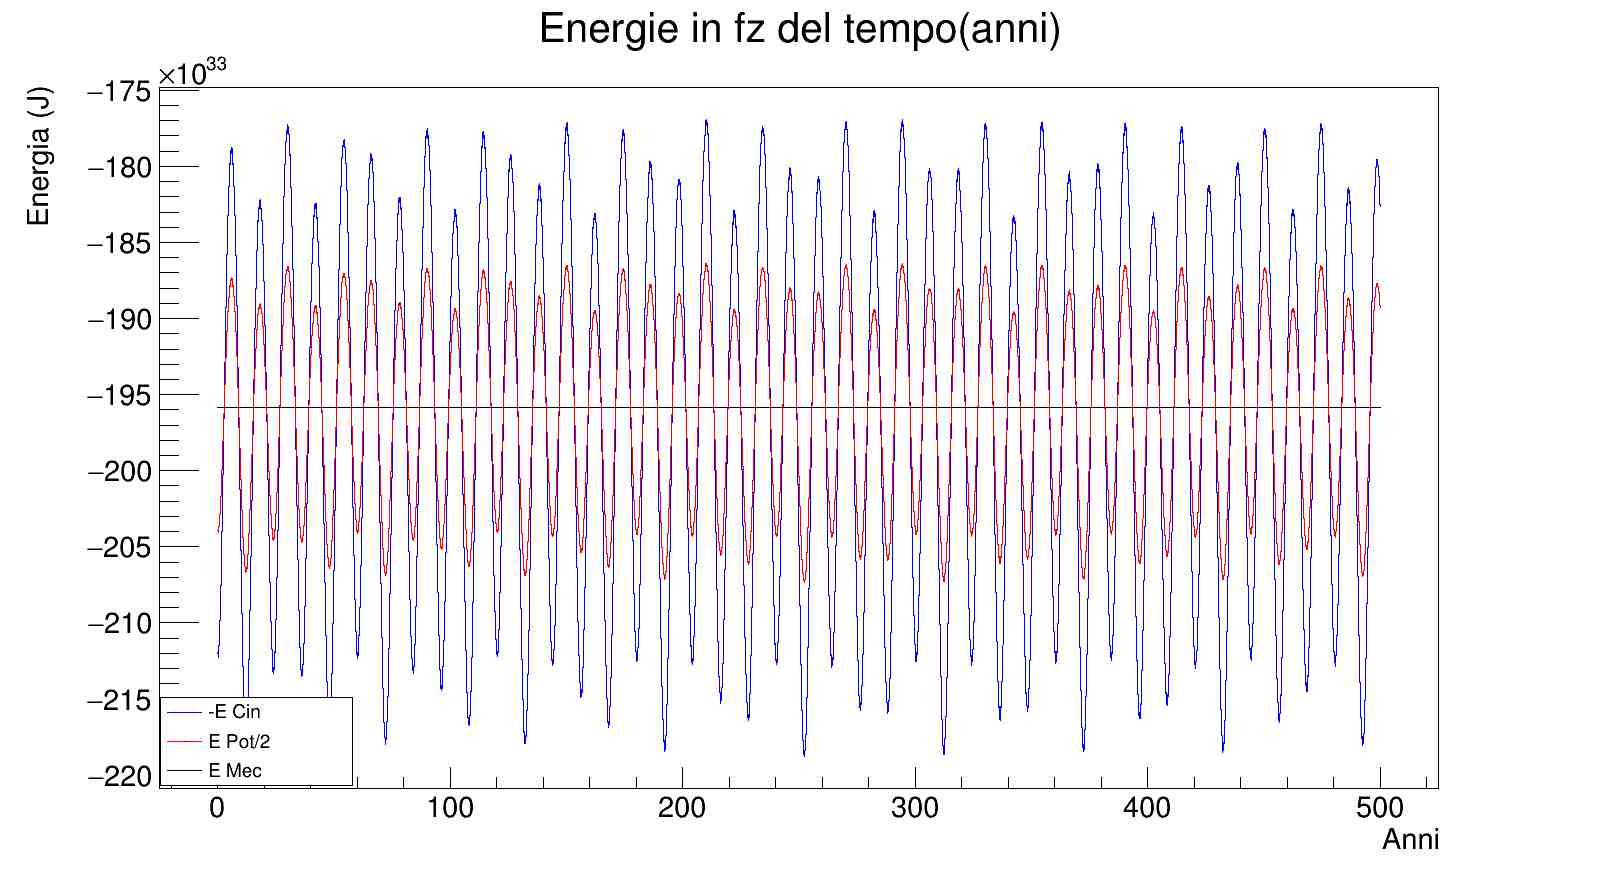
\includegraphics[width=\textwidth]{4_energia/peak/E_tempo.jpg}\\
                \label{cfr::E6T}
            \end{figure}
            Periodo Ecin= $12.030158665532817 \pm 0.1601803788742225$ anni\\
            $R^2$ = 0.9501470164550792\\
            Periodo Epot= $12.030160972927428 \pm 0.16017935829280674$ anni\\
            $R^2$ = 0.9507811667924508
        \end{frame}
        \begin{frame}{Andamenti nel tempo}
            \begin{figure}
                \centering
                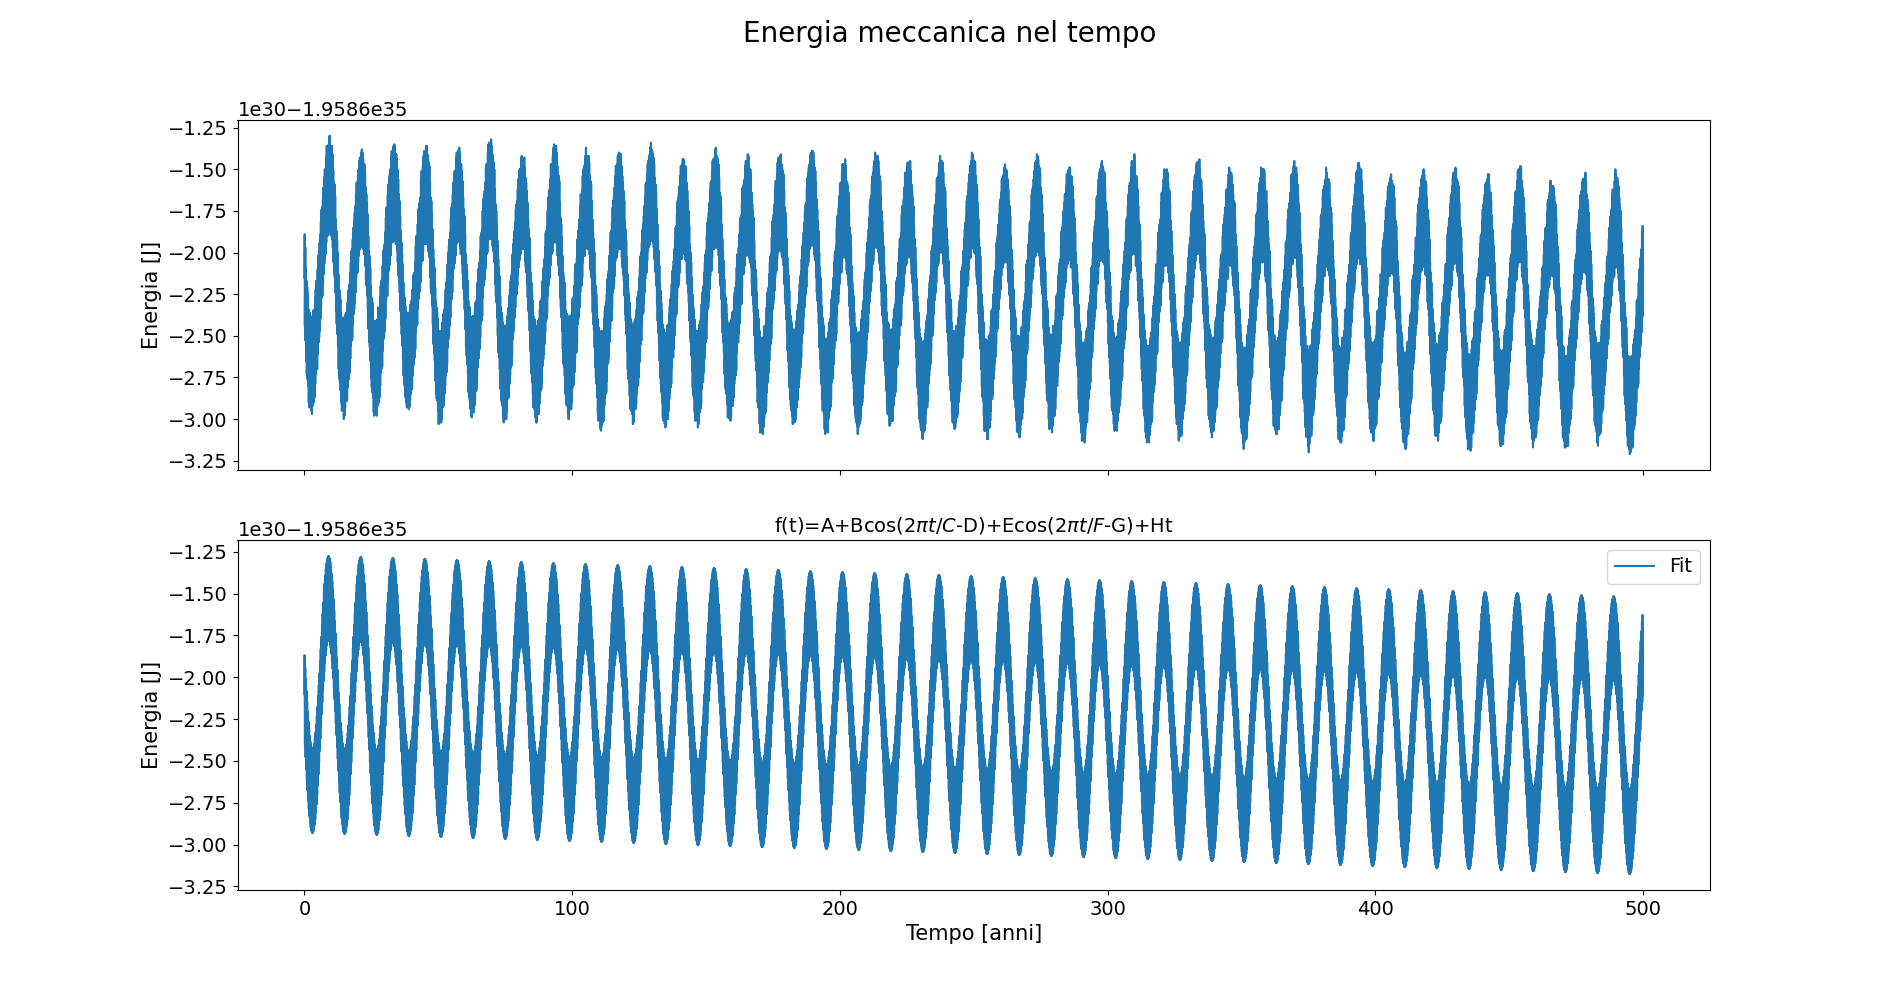
\includegraphics[width=\textwidth]{4_energia/peak/mec_500_2.png}\\
                \label{cfr::E6T}    
            \end{figure}  
            T portante= $ 12.000008934962754 \pm 0.10447251253008041$ anni\\
            Pendenza decrescita= -5e+26 Joule
        \end{frame}
        \begin{frame}{Andamenti nel tempo}
            \begin{figure}
                \centering
                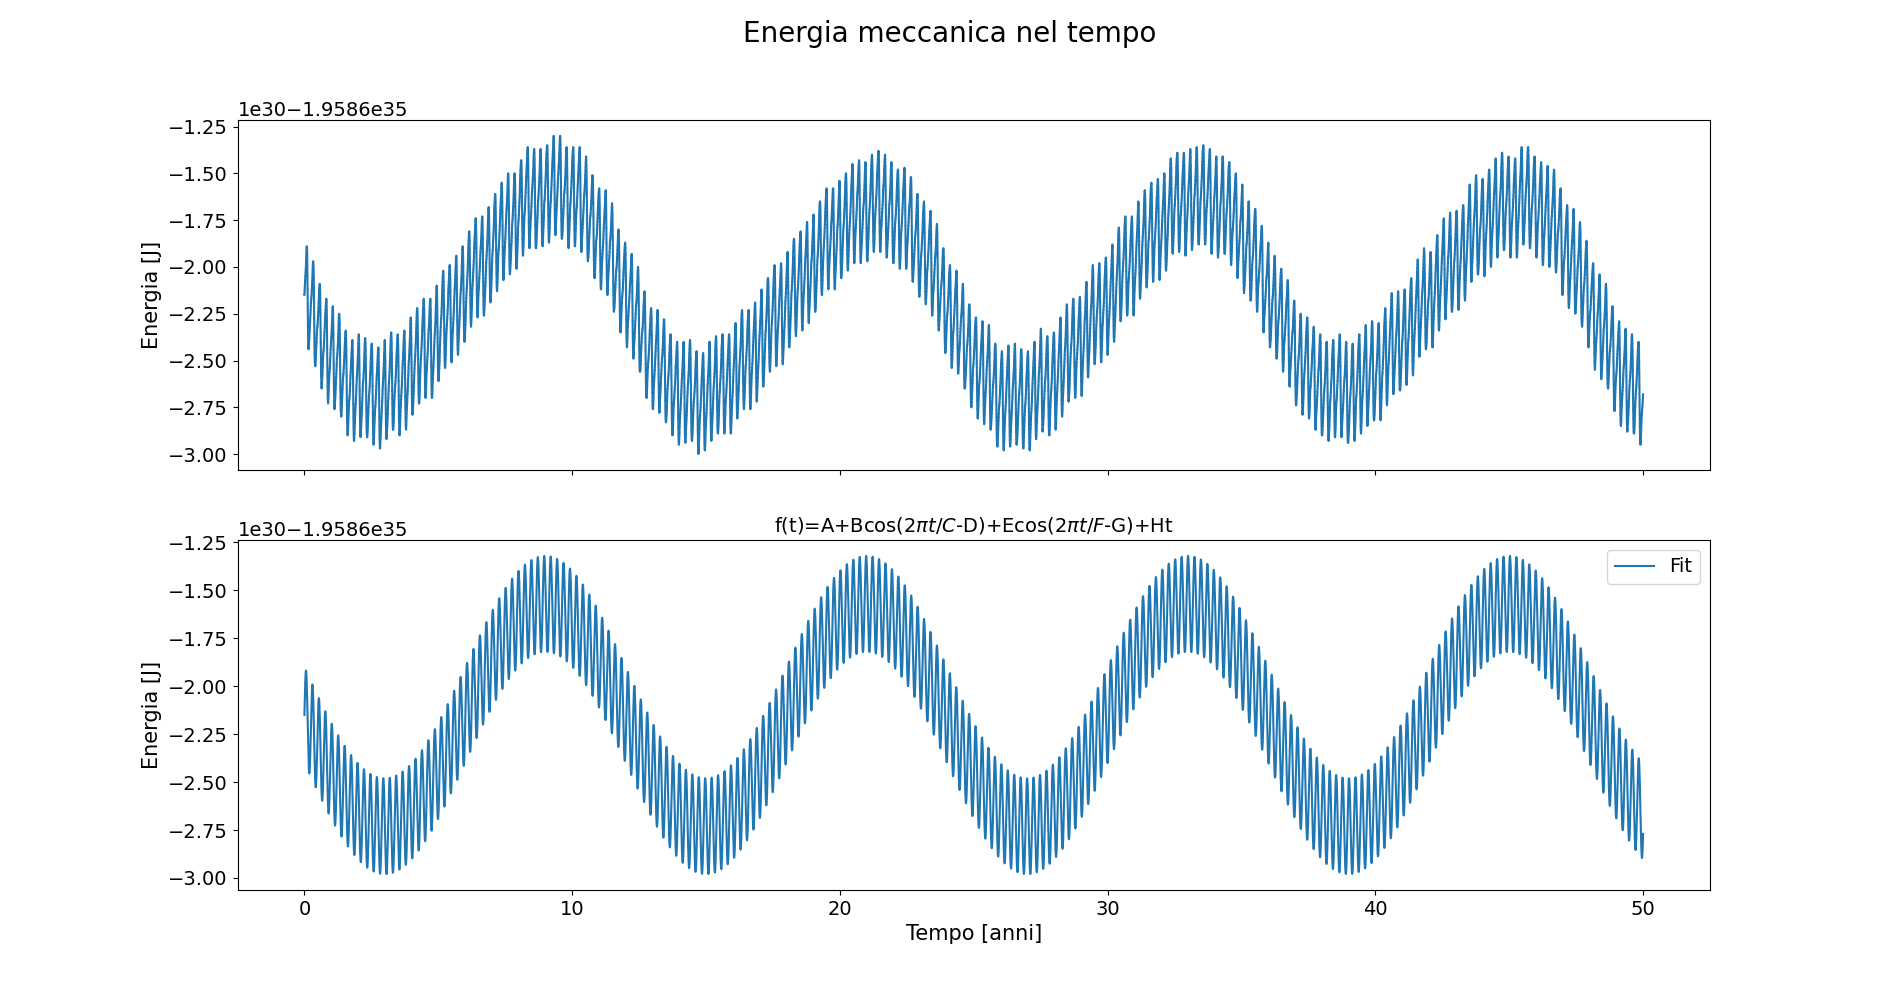
\includegraphics[width=\textwidth]{4_energia/peak/mec_50_1.png}\\
                \label{cfr::E6T}    
            \end{figure}  
            T modulante= $87.84482197184609 \pm 0.03564632637201194$ giorni\\
        \end{frame}

        \begin{frame}{Possibile spigazione}
            \begin{columns}
                \column{.5\textwidth}
                    \begin{itemize}
                        \item Influenza del moto di Giove
                        \item Il Sole non rimane fisso nell'origine
                        \item[$\Rightarrow$] Differenze tra due tratti dell'orbita di Giove
                    \end{itemize}
                \column{.5\textwidth}
                    \centering        
                    \includegraphics[width=5cm, height=3.75cm]{4_energia/peak/.jpg}\\
                    %qui grafico moto di giove 
                    \label{cfr::eme}      
            \end{columns}
            \begin{figure}
                \centering
                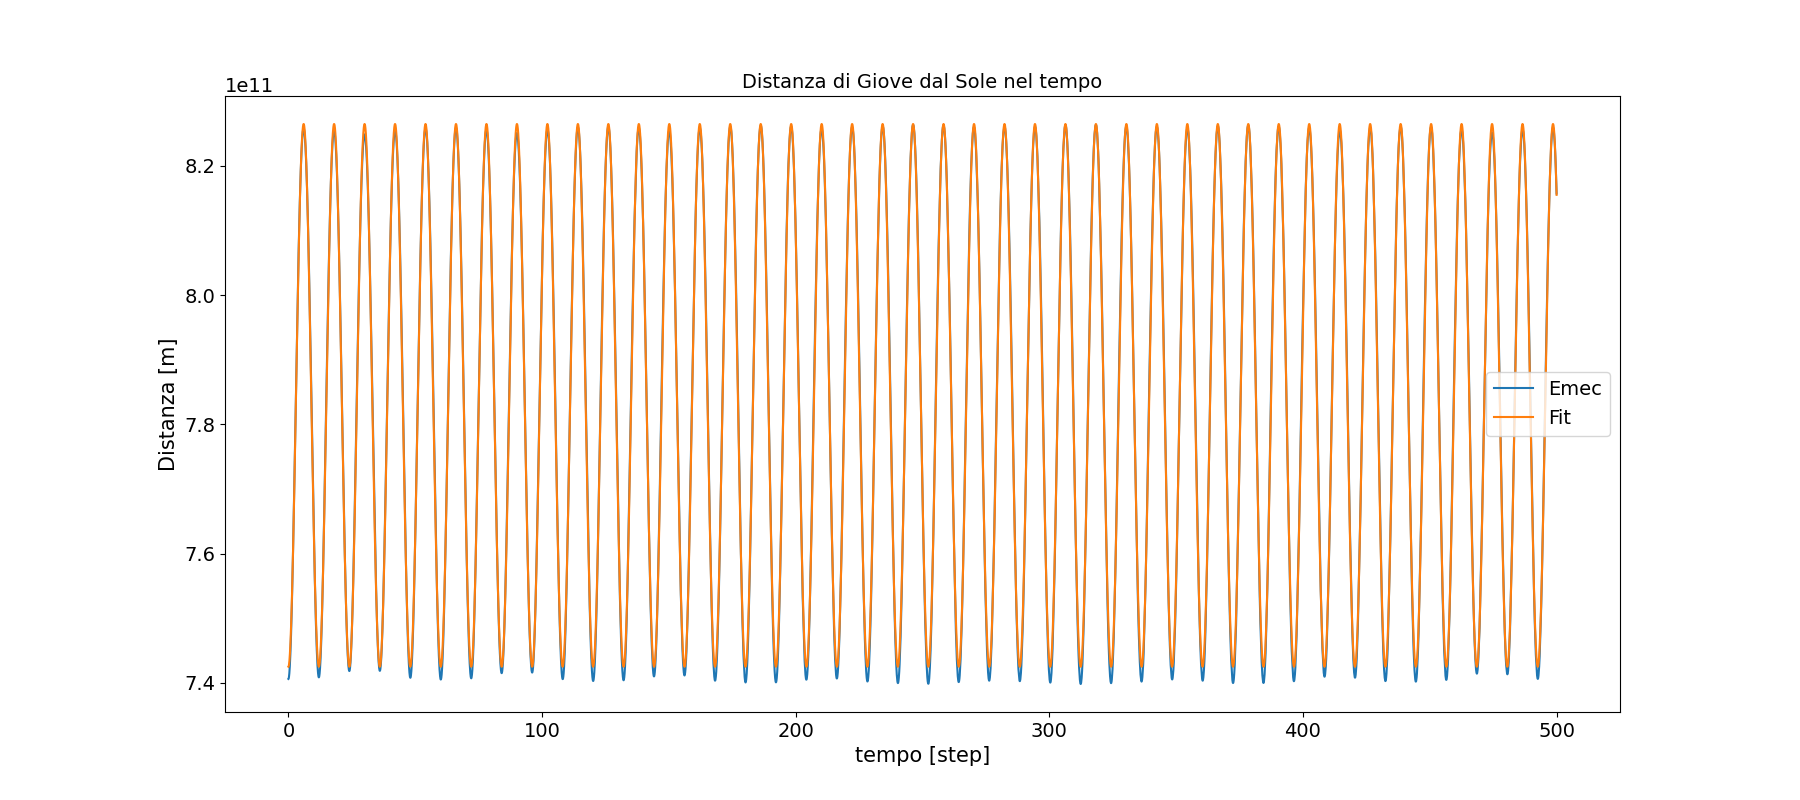
\includegraphics[height=3.75cm]{4_energia/peak/giove_fit.png}\\
            \end{figure}
        \end{frame}

        \begin{frame}{Verifica}
            \begin{columns}
                \column{.5\textwidth}
                    Simulazione con Sole fisso nell'origine del sistema di riferimento\\
                    OSS: Potrebbe spiegare anche i grafici precedenti\\
                    \vspace{1cm}
                    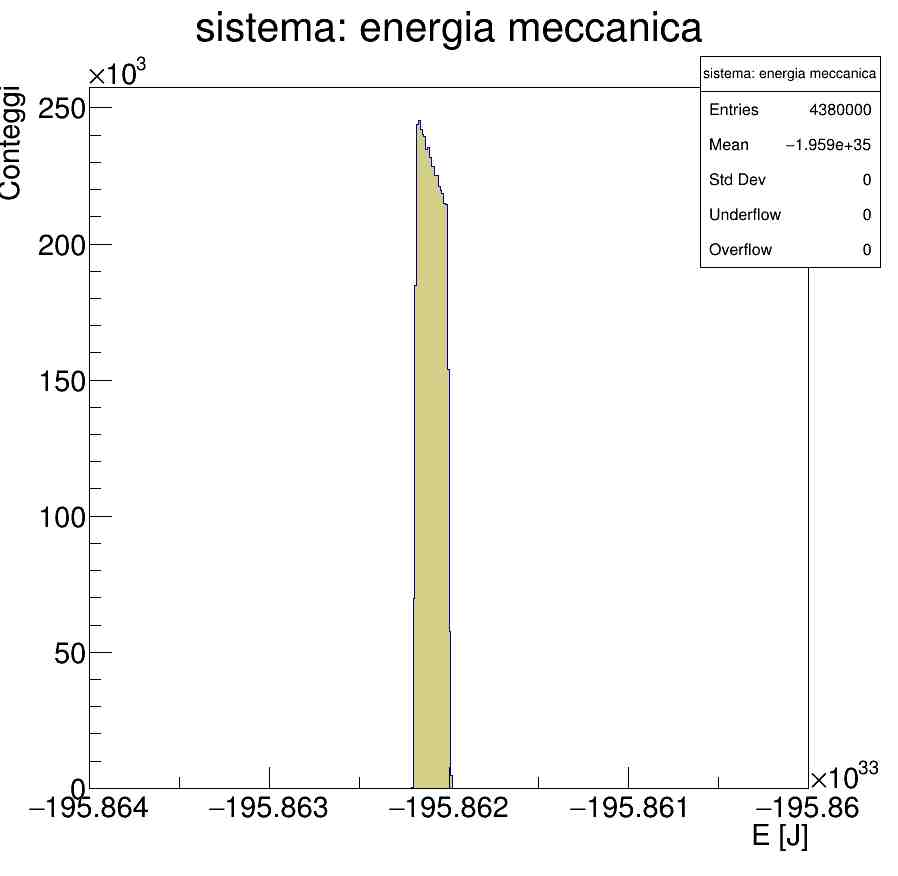
\includegraphics[width=5cm,height=3.75cm]{4_energia/peak/sf_E.jpg}\\
                \column{.5\textwidth}
                    \centering        
                    \includegraphics[width=5cm,height=3.75cm]{4_energia/peak/5000.jpg}\\
                    \includegraphics[width=5cm,height=3.75cm]{4_energia/peak/5000_tempo.jpg}
                    \label{cfr::eme}      
            \end{columns}
        \end{frame}

    
     \subsection[Dist Sole]{DIstanza dal Sole}
        \begin{frame}{Traiettorie}
            \begin{columns}
                \column{.6\textwidth}
                    %\centering
                    Nel tempo il sistema trasla $\Rightarrow$ I pianeti non compiono orbite chiuse.\\
                    Per valutare la stabilità del sistema è necessario monitorare l'andamento della distanza di ogni pianeta dal Sole, non ddall'origine del sistema di riferimento.
                    \includegraphics[width=.9\textwidth]{5_distanza/sistema_orbite.png}
                    \label{cfr::orb} 
                \column{.4\textwidth}
                    \centering
                    \includegraphics[width=.9\textwidth, height=3.75cm]{5_distanza/ter_vd_errato.jpg}
                    \includegraphics[width=.9\textwidth]{5_distanza/terra_vdds_luna.jpg}
            \end{columns}
        \end{frame}
        
        \begin{frame}{Istogramma Velocità - distanza dal Sole}
            \begin{columns}
                \column{.5\textwidth}
                    \centering
                    \includegraphics[width=.9\textwidth]{5_distanza/terra_vdds_luna.jpg}
                    \caption{Con la Luna}
                \column{.5\textwidth}
                    \centering
                    \includegraphics[width=.9\textwidth]{5_distanza/terra_vds_noluna.jpg}
                    \caption{Senza Luna}
            \end{columns}
        \end{frame}
        \begin{frame}{Istogramma Velocità - distanza dal Sole}
            \begin{columns}
                \column{.5\textwidth}
                    \centering
                    \includegraphics[width=.9\textwidth]{5_distanza/terra_vds_solefisso_luna.jpg}
                    \caption{Con il Sole fisso e la Luna}
                \column{.5\textwidth}
                    \centering
                    \includegraphics[width=.9\textwidth]{5_distanza/terra_vds_solefisso_noluna.jpg}
                    \caption{Con il Sole fisso e senza Luna}
            \end{columns}
        \end{frame}
        
        \begin{frame}{Distanza vs posizioni iniali}
            \begin{columns}
                \column{.35\textwidth}
                    In questo caso risultati differenti a seconda del pianeta:
                    \begin{enumerate}
                        \item Nettuno - ottimale con dati perielio
                    \end{enumerate}
                \column{.65\textwidth}
                    \centering
                    \includegraphics[width=\textwidth]{5_distanza/Net_epri_500.jpg}
                    \includegraphics[width=\textwidth]{5_distanza/net_afe_500.jpg}
                    \caption{Dati perielio(in alto) e dati afelio(sotto)}
                    \label{cfr::net} 
            \end{columns}
        \end{frame}
        \begin{frame}{Distanza vs posizioni iniali}
            \begin{columns}
                \column{.35\textwidth}
                    In questo caso risultati differenti a seconda del pianeta:
                    \begin{enumerate}
                        \item Nettuno - ottimale con dati perielio
                        \item Venere - sempre leggermente fuori misura
                    \end{enumerate}
                \column{.65\textwidth}
                    \centering
                    \includegraphics[width=\textwidth]{5_distanza/Ven_peri_500.jpg}
                    \includegraphics[width=\textwidth]{5_distanza/Ven_afe_500.jpg}
                    \caption{Dati perielio(in alto) e dati afelio(sotto)}
                    \label{cfr::ven} 
            \end{columns}
        \end{frame}
        \begin{frame}{Distanza vs posizioni iniali}
            \begin{columns}
                \column{.35\textwidth}
                    In questo caso risultati differenti a seconda del pianeta:
                    \begin{enumerate}
                        \item Nettuno - ottimale con dati perielio
                        \item Venere - sempre leggermente fuori misura
                        \item tutti errati con dati medi
                    \end{enumerate}
                \column{.65\textwidth}
                    \centering
                    \includegraphics[width=\textwidth]{5_distanza/terra_medi.jpg}
                    \includegraphics[width=\textwidth]{5_distanza/mototera_500.jpg}
                    \label{cfr::Terra} 
                    \caption{Dati medi(in alto) e dati mix(sotto)}
            \end{columns}
        \end{frame}
        \begin{frame}{Distanza vs T e deltaT}
            \begin{figure}
                \centering
                \includegraphics[width=\textwidth, height=3.75cm]{5_distanza/ven_8000_drift.jpg}\\
                \includegraphics[width=\linewidth, height=3.75cm]{5_distanza/sat_moto_afe_bug_50k_3600.jpg}
                %\caption{Caption}
                \label{fig:8000}
            \end{figure}
        \end{frame}
        \begin{frame}{Grafici con Python}
            \begin{columns}
                \column{.5\textwidth}
                    \centering        
                    \includegraphics[width=5cm,height=5cm]{5_distanza/ura_orbita.png}      
                \column{.5\textwidth}
                    \centering        
                    \includegraphics[width=5cm,height=3.75cm]{5_distanza/gio_osc_500_bello.png}\\
                    \includegraphics[width=5cm,height=3.75cm]{5_distanza/gio_osc_500_bello.png} 
            \end{columns}
        \end{frame}
    
        \subsection{Eccentricità}
        \begin{frame}{Calcolo dell'eccentricità}
            \begin{columns}
                \column{.4\textwidth}
                    \begin{equation}
                        e = \sqrt{1+\frac{2EL^2}{m_r\alpha^2}}
                    \end{equation}
                    Con
                    \begin{itemize}
                        \item E: energia orbitale*
                        \item L: momento angolare orbitale
                        \item $m_r=\frac{Mm}{m+M}$: massa ridotta del sistema
                        \item $\alpha = F r^2 = GMm$
                    \end{itemize}
                    \small *solo interazione gravitazionale col Sole
                \column{.6\textwidth}
                    \centering
                    \includegraphics[width=.9\textwidth, height=3.75cm]{6_ecc/.jpg}
                    %mettigrafico buggato di mercurio
                    \includegraphics[width=.9\textwidth, height=3.75cm]{6_ecc/mar_ecc_bug.jpg}
                    \label{cfr::bug} 
            \end{columns}
        \end{frame}
        \begin{frame}{Calcolo dell'eccentricità - correzione}
            \begin{columns}
                \column{.4\textwidth}
                    \begin{equation}
                        e = \sqrt{1+\frac{2EL^2}{m_r\alpha^2}}
                    \end{equation}
                    Con
                    \begin{itemize}
                        \item E: energia orbitale*
                        \item L: momento angolare rispetto al sole - eliminiamo la componente di traslazione del sistema
                        \item $m_r=\frac{Mm}{m+M}$: massa ridotta del sistema
                        \item $\alpha = F r^2 = GMm$
                    \end{itemize}
                    \small *solo interazione gravitazionale col Sole
                \column{.6\textwidth}
                    \centering
                    \includegraphics[width=.9\textwidth, height=3.75cm]{6_ecc/mer_ecc_500_3600.jpg}
                    \includegraphics[width=.9\textwidth, height=3.75cm]{6_ecc/net_ecc_500_60.jpg}
                    \label{cfr::bug3} 
            \end{columns}
        \end{frame}
        \begin{frame}{Eccentricità - dipendenza dai parametri}
            \begin{block}{Risultati molto più piccati ma fortemente dipendenti dalle condizioni, non sempre corretti:}
                \begin{itemize}
                    \item Terra e Venere: valori sempre lontani da quelli reali
                    \item Altri pianeti:
                    \begin{itemize}
                        \item Afelio: valori compatibili tra simulazioni con diversi T e deltaT, ma bassi rispetto a quelli reali
                        \item Perielio: valori compatibili tra simulazioni con diversi T e deltaT, ma alti rispetto a quelli reali per quasi tutti i pianeti
                        \item Mix: valori compatibili tra simulazioni con diversi T e deltaT, compatibili anche col valore reale fino a qualche migliaia di anni
                    \end{itemize}
                \end{itemize}               
            \end{block}
            \begin{table}[]
                \centering
                \begin{tabular}{c|ccc|c}
                    500/3600 & Afelio & Prielio & Mix & Reale \\
                    \hline
                    Mercurio & 0.201473 & 0.212235 & 0.202448 & 0.2056 \\
                    Terra & \textbf{0.0119076} &\textbf{ 0.0219439} & 0.0134867 & 0.0167 \\
                    Giove & \textbf{0.0297916} & 0.046467 & 0.0470972 & 0.0484 \\
                    Nettunp & 0.00735812 & \textbf{0.0132255} & 0.00734893 & 0.0086 \\
                \end{tabular}
                %\caption{Caption}
                \label{tab:ecce}
            \end{table}
        \end{frame}

            \subsubsection[Fix]{Sole fisso}
        \begin{frame}{NOTA - Simulazioni con sole fermo}
            \begin{columns}
                \column{.5\textwidth}
                    \centering
                    \includegraphics[width=\textwidth, height=3.75cm]{14_fisso/sf_Ltot.jpg}\\
                    \includegraphics[width=\textwidth, height=3.75cm]{14_fisso/.jpg}
                    %metti grafico eccentricità
                \column{.5\textwidth}
                    \centering
                    \includegraphics[width=\textwidth]{14_fisso/sf_terra_ok.jpg}\\\
                    \includegraphics[width=\textwidth]{}     
            \end{columns}
        \end{frame}
        \begin{frame}{NOTA - Simulazioni con sole fermo}
            Deriva per tempi lunghi
            \vspace{1cm}
            \begin{columns}
                \column{.5\textwidth}
                    \centering
                    \includegraphics[width=\textwidth]{14_fisso/sf_5k_sat_orb.jpg}  
                \column{.5\textwidth}
                    \centering
                    \includegraphics[width=\textwidth]{14_fisso/sf_5k_sat_drift.jpg}   
            \end{columns}
        \end{frame}
    
        \subsection[\theta]{Inclinazione orbita}
        \begin{frame}{Orbite 3D}
            \begin{columns}
                \column{.45\textwidth}
                    \begin{block}{Modifiche al codice}
                        \begin{enumerate}
                            \item modifiche ai file di configurazione e alla funzione sistema::leggi()
                            \item aggiunta funzione vettore::angolo() per il calcolo dell'angolo tra due vettori nello spazio
                            \item inserimento del codice seguente nella funzione corpo::evolvidt()
                            \begin{enumerate}[i]
                                \item calcolo dell'angolo ad ogni step rispetto a piano eclittica istantaneo
                                \item raccolta dati in istogramma
                            \end{enumerate}
                        \end{enumerate}
                    \end{block}
                \column{.55\textwidth}
                    %\centering
                    %da sistemare - voglio mettere codice
                    %\includegraphics[width=.9\textwidth]{7_incli/code.png}
                    \begin{lstlisting}[language=C++]
//valuto inclinazione 
corpo *terra=cc[3]; 
vettore tp=terra->P(); 
vettore dtt=tp-sp; 
vettore vt=terra->V(); 
vettore nt=dtt*vt; 
if(m_nome!="Luna") 
    m_teta=90-ds.angolo(nt); 
else{ 
    vettore lt=m_pos-tp; 
    m_teta=90-lt.angolo(nt); 
}
\end{lstlisting}
            \end{columns}
        \end{frame}
        
        \begin{frame}{Orbite 3D - stabili nei limiti evidenziati sopra}
            \begin{columns}
                \column{.5\textwidth}
                    \centering        
                    \includegraphics[width=5cm,height=3.75cm]{7_incli/ven_incl_500_3600.jpg}\\
                    \includegraphics[width=5cm,height=3.75cm]{7_incli/lun_incl_600_60.jpg}
                    \label{cfr::vin}              
                \column{.5\textwidth}
                    \centering        
                    \includegraphics[width=5cm,height=3.75cm]{7_incli/gio_inc_temp_500_3600.jpg}\\
                    \includegraphics[width=5cm,height=3.75cm]{7_incli/ura_inc_bug_50k_3600.jpg}
                    \label{cfr::sdf}
            \end{columns}
        \end{frame}
        
        \begin{frame}{Grafici con Python}
            \begin{columns}
                \column{.5\textwidth}
                    \centering        
                    \includegraphics[width=5cm,height=3.75cm]{7_incli/ven_teta.png}\\
                    \label{cfr::in}              
                \column{.5\textwidth}
                    \centering        
                    \includegraphics[width=5cm,height=3.75cm]{7_incli/sat_teta_tempo.png}\\
            \end{columns}
        \end{frame}

\section[Valid]{Validazione}
    \begin{frame}
        \frametitle{Contenuti}
        \transblindsvertical
        \tableofcontents[currentsection]
    \end{frame}
    
        \subsection[Sim]{Simulazione con 2 corpi}
        \begin{frame}{2 corpi - Stabilità dopo 50000 anni}
            \begin{columns}
                \column{.5\textwidth}
                    \centering        
                    \includegraphics[width=5cm,height=3.75cm]{13_2cc/ura_Ltot.jpg}\\
                    \includegraphics[width=5cm,height=3.75cm]{13_2cc/ura_ecc.jpg}
                    \label{cfr::vin}              
                \column{.5\textwidth}
                    \centering        
                    \includegraphics[width=5cm,height=3.25cm]{13_2cc/ura_teta_tempo.jpg}\\
                    \includegraphics[width=5cm,height=3.25cm]{13_2cc/ven_drift.jpg}
                    \caption{Deriva di Venere (e Mer)}
                    \label{cfr::sdf}
            \end{columns}
        \end{frame}

        \subsection[Analitic]{Soluzione analitica}
        \begin{frame}{Algoritmo}
            \begin{block}
                \begin{enumerate}
                    \item prendo intervallo uniforme di angoli tra 0 e 2
                    \item calcolo i tempi associati e la distanza
                    \item replico gli array il numero di periodi necessario
                    \item dal dataset dei tempi-distanze seleziono d corrispondenti
                    \item plotto questi due dataset e la loro differenza per vedere come varia nel tempo
                \end{enumerate}
            \end{block}
            \begin{equation}
                e = \sqrt{1+\frac{2EL^2}{m_r\alpha^2}}
            \end{equation}
        \end{frame}

\section[Code II]{Questioni tecniche}
    \begin{frame}
        \frametitle{Contenuti}
        \transblindsvertical
        \tableofcontents[currentsection]
    \end{frame}
    
    \begin{frame}{Efficienza}
        \begin{exampleblock}{Gestione ROOT::TGraph}
            \begin{enumerate}
                \item Raccolta dati
                \begin{enumerate}[a]
                    \item Aggiunta punti ad ogni iterazione - analogo agli istogrammi
                    \item Utilizzo di array
                    \item Raccolta dati in file txt separati per ogni pianeta
                    \item Raccolta dati in file txt unico
                \end{enumerate}
            \end{enumerate}
            \vspace{3mm}}}
            Problemi:
            \begin{enumerate}[i]
                \item Evitare crash del programma per eccessiva occpuazione di memoria (perdita dati simulaziuone)
                \item Limitare il tempo di esecuzione
            \end{enumerate}
        \end{exampleblock}
    \end{frame}
    
    \begin{frame}{Efficienza}
        \begin{exampleblock}{Gestione ROOT::TGraph}
            \begin{enumerate}
                \item Raccolta dati
            \end{enumerate}
            \vspace{3mm}
            Problemi:
            \begin{enumerate}[i]
                \item Evitare crash del programma per eccessiva occpuazione di memoria (perdita dati simulazione)
                \item Limitare il tempo di esecuzione
            \end{enumerate}
            \vspace{3mm}
            \textit{Soluzione migliore}:
            \begin{itemize}
                \item Raccolta dati in unico file con formattazione in colonne
                \item Creazione e visualizzazione dei grafici opzionale
                \item Campionamento dati
                \item Salvataggio istogrammi in file esterno
            \end{itemize}
        \end{exampleblock}
    \end{frame}

    \begin{frame}{Efficienza}
        \begin{exampleblock}{Gestione ROOT::TGraph}
            \begin{enumerate}
                \item Raccolta dati
                \item Visualizzazione
            \end{enumerate}
            \vspace{3mm}
            Problemi:
            \begin{enumerate}[i]
                \item Conflitto con ROOT::THI
            \end{enumerate}
            \vspace{3mm}
            \textit{Soluzione}: Spostamento definizione del ROOT::TCanvas\\
            \begin{lstlisting}
TApplication myApp("App", &argc, argv);
TCanvas *screen2 = new TCanvas("c1", 
    "My Solar System", 0, 0, 900, 900);

sistema s(nAnni, ddt, confFile, outFile);
\end{lstlisting}
        \end{exampleblock}
    \end{frame}

    \begin{frame}{Python}
        \begin{block}{Contro}
            \begin{enumerate}
                \item Dati salvati sempre in np.array $\Rightarrow$ Enorme consumo di memoria che aumenta col tempo - 43% di RAM per la simulazione "standard"
                \item Creazione e plot di istogrammi e grafici richiede ancor più memoria che C++
                \item Tempo di esecuzione enormemente più grande - 2.5 ore per la simulazione "standard"
            \end{enumerate}          
        \end{block}
        \begin{block}{Pro}
            \begin{enumerate}
                \item Migioor resa grafica
                \item Scrittura più agevole del codice e funzionalità aggiunbtive
            \end{enumerate}
        \end{block}
        $\Rightarrow$ Utilizzato per analisi dati e confronto tra diverse simulazioni svolte con C++
    \end{frame}

%\section{Precessione}
    \begin{frame}
        \frametitle{Contenuti}
        \transblindsvertical
        \tableofcontents[currentsection]
    \end{frame}
    
    \begin{frame}{Calcolo della precessione}
        \begin{columns}
            \column{.5\textwidth}
                \begin{enumerate}
                    \item Individuazione perielio
                    \item Calcolare angolo con la posizione precedente del perielio - otteniamo $\frac{angolo}{periodo\ orbitale}$
                    \item Iterare il procedimento
                    \item Calcolare media e deviazione standard
                    \item Convertire in $\frac{arcsec}{anno\ terrestre}$ per confrontare coi adti reali
                \end{enumerate}
            \column{.5\textwidth}
                \centering
                \includegraphics[width=.9\textwidth]{9_prec/precessione.png} \\
                \vspace{3mm}
                \includegraphics[width=.9\textwidth]{9_prec/mercurio.png}
        \end{columns}
    \end{frame}

    \begin{frame}{Modifiche al codice}
        \begin{block}{}
        \begin{enumerate}
            \item File di configurazione - aggiunta periodi rivoluzione pianeti
            \item classe Corpo Celeste  -
            \begin{enumerate}[a]
                \item Aggiunta membri m\_TT e m\_peri
                \item Modifiche a evolvidT()
                \item Correzione relativistica al calcolo dell'accelerazione
                \item Aggiunta funzione precessione() per l'analisi dei dati
                \item Aggiunta altri membri e metodi di servizio 
            \end{enumerate}
        \end{enumerate}
        \end{block}
        \begin{equation}
            \vec{a_i} = -\sum_{i\neq j}\frac{Gm_j}{r_{ij}^2}(1+\beta\frac{r_L^2}{r_{ij}^2})\frac{\vec r_{ij}}{r_{ij}}\,\,\,\,\,\,\,\,\forall i=1,\dots N
        \end{equation}
        \centering
        Con $\beta=3$ e $\vec{r_L}=\frac{\vec{L}}{mc}=\frac{\vec{r_{ij}}\times\vec{v_j}}{c}$
        %\begin{lstlisting}[language=C++]
void corpo::precessione(float Tterra){
    if(m_nome=="Sole")m_histos[7]->Fill(0);
    else{
        for(int i=1; i<m_peri.size(); i++){
            m_histos[7]->Fill
                (m_peri[i].angolo(m_peri[i-1])
                    *Tterra/m_TT);
        }
    }
}
\end{lstlisting}            
    \end{frame}

    \begin{frame}{Modifiche a corpo::evolvidT( ... ) - v1}
        \begin{lstlisting}[language=C++]
    [...]
    corpo sole*=cc[0];
    vettore sp=sole->P();
    float dSole=(m_pos-sp).modulo();
    [...]
    if(m_nome!="Sole"){
        float d_cfr=(m_app-m_sap).modulo();
        if(dSole<d_cfr){
            m_app=m_pos;
    	m_sap=sp;
        }
        uint64_t Tstep = m_TT *24*3600 / dt ;
        if((j+1)%Tstep == 0){
    	m_peri.push_back(m_app-m_sap);
    	m_app=m_pos;
    	m_sap=sp;
        }
    }
\end{lstlisting}
    \end{frame}
    \begin{frame}{Modifiche a corpo::evolvidT( ... ) - v2}
        \begin{lstlisting}[language=C++]
    corpo sole*=cc[0];
    if(m_nome=="Sole" && j<2){
	m_app=vettore(0,0,0);
    }
    else{
	m_app=m_pos0;
	m_sap=m_s0;
    }	
    m_s0=sole->P0();
    m_pos0=m_pos; [...]
    vettore sp=sole->P();
    float dSole=(m_pos-sp).modulo();
    if(m_nome!="Sole"){
	float d_media=(m_pos0-m_s0).modulo();
	float d_pre=(m_app-m_sap).modulo();
	if(d_media<d_pre && d_media<dSole)
		m_peri.push_back(m_pos0-m_s0);
    }
\end{lstlisting}
    \end{frame}

    \begin{frame}{Risultati (Obiettivo $= 56 \frac{arcsec}{anno\ terrestre}$)}
        Forte disaccordo coi dati reali:
        \vspace{3mm}
        \begin{columns}
            \column{.4\textwidth}
                \centering
                Senza Relatività
                \includegraphics[width=\textwidth, height=3cm]{9_prec/sballati/10_3600_nor_1.jpg}\\
                \includegraphics[width=\textwidth, height=3cm]{9_prec/sballati/10_60_nor_1.jpg}
            \column{.2\textwidth}
                \centering
                10a/3600s\\
                \vspace{3cm}
                10a/60s
            \column{.4\textwidth}
                \centering
                Con Relatività
                \includegraphics[width=.9\textwidth, height=3cm]{9_prec/sballati/10_3600_rel_1.jpg}\\
                \includegraphics[width=.9\textwidth, height=3cm]{9_prec/sballati/10_60_rel_1.jpg}
        \end{columns}
    \end{frame}
    \begin{frame}{Risultati (Obiettivo $= 56 \frac{arcsec}{anno\ terrestre}$)}
        \begin{columns}
            \column{.4\textwidth}
                \centering
                Senza Relatività
                \includegraphics[width=\textwidth, height=3.25cm]{9_prec/sballati/100_3600_nor_1.jpg}\\
                \includegraphics[width=\textwidth, height=3.25cm]{9_prec/sballati/100_600_nor_1.jpg}
            \column{.2\textwidth}
                \centering
                100a/3600s\\
                \vspace{3cm}
                100a/600s
            \column{.4\textwidth}
                \centering
                Con Relatività
                \includegraphics[width=\textwidth, height=3.25cm]{9_prec/sballati/100_3600_rel_1.jpg}\\
                \includegraphics[width=\textwidth, height=3.25cm]{9_prec/sballati/100_600_rel_1.jpg}
        \end{columns}
    \end{frame}
    \begin{frame}{Risultati (Obiettivo $= 56 \frac{arcsec}{anno\ terrestre}$)}
        \begin{columns}
            \column{.4\textwidth}
                \centering
                Senza Relatività
                \includegraphics[width=\textwidth, height=3.25cm]{9_prec/sballati/10_6_nor_1.jpg}\\
                \includegraphics[width=\textwidth, height=3.25cm]{9_prec/sballati/500_3600_nor_1.jpg}
            \column{.2\textwidth}
                \centering
                10a/6s
                \vspace{3cm}
                500a/3600s
            \column{.4\textwidth}
                \centering
                Con Relatività
                \includegraphics[width=\textwidth, height=3.25cm]{9_prec/sballati/10_6_rel_1.jpg}\\
                \includegraphics[width=\textwidth, height=3.25cm]{9_prec/sballati/500_3600_rel_1.jpg}
        \end{columns}
    \end{frame}

    \begin{frame}{Risultati (Obiettivo $= 56 \frac{arcsec}{anno\ terrestre}$)}
        \begin{columns}
            \column{.4\textwidth}
                \centering
                Con Relatività solo rispetto al sole
                \includegraphics[width=\textwidth, height=3.25cm]{9_prec/sballati/10_3600_relB_1.jpg}\\
                \includegraphics[width=\textwidth, height=3.25cm]{9_prec/sballati/100_600_relB_1.jpg}
            \column{.2\textwidth}
                \centering
                10a/3600s\\
                \vspace{3cm}
                100a/600s
            \column{.4\textwidth}
                \centering
                Con Relatività
                \includegraphics[width=\textwidth, height=3.25cm]{9_prec/sballati/10_3600_rel_1.jpg}\\
                \includegraphics[width=\textwidth, height=3.25cm]{9_prec/sballati/100_600_rel_1.jpg}
        \end{columns}
    \end{frame}

%\section[Approx II]{Ordini Superiori}
%    \begin{frame}
%        \frametitle{Contenuti}
%        \transblindsvertical
%        \tableofcontents[currentsection]
%    \end{frame}
    
%    \subsection[Algo II]{Algoritmi}
    \begin{frame}{Altri algoritmi}
        \begin{exampleblock}{$N>2 \Rightarrow$ Soluzione approssimata tramite metodi iterativi discreti:}
            \begin{enumerate}
                \item Runge-Kutta $2^{nd}$ order - altra versione
            \end{enumerate}
        \end{exampleblock}
        devo aggiungere formule metodo
    \end{frame}
    \begin{frame}{Altri algoritmi}
        \begin{exampleblock}{$N>2 \Rightarrow$ Soluzione approssimata tramite metodi iterativi discreti:}
            \begin{enumerate}
                \item Runge-Kutta $2^{nd}$ order - altra versione
                \item Velocity Verlet - sempre approssimazione del secondo ordine
            \end{enumerate}
        \end{exampleblock}
    \end{frame}
    \begin{frame}{Altri algoritmi}
        \begin{exampleblock}{$N>2 \Rightarrow$ Soluzione approssimata tramite metodi iterativi discreti:}
            \begin{enumerate}
                \item Runge-Kutta $2^{nd}$ order - altra versione
                \item Velocity Verlet - sempre approssimazione del secondo ordine
                \item Runge-Kutta $4^{th}$
            \end{enumerate}
        \end{exampleblock}
    \end{frame}
    \begin{frame}{Altri algoritmi}
        \begin{exampleblock}{$N>2 \Rightarrow$ Soluzione approssimata tramite metodi iterativi discreti:}
            \begin{enumerate}
                \item Runge-Kutta $2^{nd}$ order - altra versione
                \item Velocity Verlet - sempre approssimazione del secondo ordine
                \item Runge-Kutta $4^{th}$
                \item Yoshida $4^{th}$ order - algoritmo del quarto ordine
            \end{enumerate}
        \end{exampleblock}
    \end{frame}

%    \subsection[Effetti]{Effetti sulla precessione}
    \begin{frame}{Effetti sulla precessione}
        Per ora nessun miglioramento
    \end{frame}

%    \subsection[Cfr]{Confronti su altri parametri}
    \begin{frame}{Distanza dal sole nel tempo}
        
    \end{frame}

\end{document}